\documentclass[11pt,a4paper,oneside]{book}
\usepackage[utf8]{inputenc}
\usepackage{amsmath}
\usepackage{dsfont}
\usepackage{listings}
\usepackage{amsfonts}
\usepackage{amssymb}
\usepackage{tabularx}
\usepackage{enumitem}
\usepackage{algorithm}% http://ctan.org/pkg/algorithm
\usepackage[noend]{algorithmic}
\usepackage{parskip}
\usepackage{tikz}
\usepackage[margin=1in]{geometry}
\usepackage{graphicx}
\usepackage{hyperref}
\usepackage{epigraph}
\usetikzlibrary{arrows,positioning} 
\usepackage{subcaption}
\usepackage[colorinlistoftodos]{todonotes}
\usepackage{natbib}
\usepackage{wrapfig}

\graphicspath{ {figures/} }
\pgfarrowsdeclarecombine{ring}{ring}{}{}{o}{o}

\DeclareMathOperator{\ringarrow}{\raisebox{0.5ex}{\tikz[baseline]{\draw[ring->](0,0)--(2em,0);}}}
\DeclareUnicodeCharacter{00A0}{ }
\tikzset{
    %Define standard arrow tip
    >=stealth',
    %Define style for boxes
    observed/.style={
           circle,
           rounded corners,
           draw=black, thick,
           minimum width=2.2em,
           minimum height=2.2em,
           font=\footnotesize,
           text centered,
           },
     latent/.style={
           circle,
           rounded corners,
           draw=black, thick, dashed,
           minimum width=2.2em,
           minimum height=2.2em,
           font=\footnotesize,
           text centered,
           fill=black!10!white
           },
    target/.style={
           circle,
           rounded corners,
           draw=black, thick,
           minimum width=2.2em,
           minimum height=2.2em,
           font=\footnotesize,
           text centered,
           fill=black!20!white,
           },
    observedrect/.style={
           rectangle,
           rounded corners,
           draw=black, thick,
           minimum width=6em,
           minimum height=2em,
           font=\footnotesize,
           text centered,
           },
     targetrect/.style={
           rectangle,
           rounded corners,
           draw=black, thick,
           minimum width=6em,
           minimum height=2em,
           font=\footnotesize,
           text centered,
           fill=black!20!white,
           },
     empty/.style={
           circle,
           rounded corners,
           minimum width=.5em,
           minimum height=.5em,
           font=\footnotesize,
           text centered,
           },
    % Define arrow style
    pil/.style={
           o->,
           thick,
           shorten <=2pt,
           shorten >=2pt,},
    sh/.style={ shade, shading=axis, left color=red, right color=green,
    shading angle=45 }   
}





\newcommand{\KL}{\operatorname{KL}}
\newcommand{\simpleregret}{R_T}
\newcommand{\Pij}[1]{\operatorname{P}_{ij}\!\left\{#1\right\}}
\newcommand{\Pkl}[1]{\operatorname{P}_{kl}\!\left\{#1\right\}}
\newcommand{\Q}[1]{\operatorname{Q}\left\{#1\right\}}
\newcommand{\EE}{\mathbb E}
\newcommand{\EEa}{\EE_a}
\newcommand{\Pns}[2]{\operatorname{P}_{#1}\left\{#2\right\}}
\newcommand{\Pn}[2]{\operatorname{P}\left\{#2|#1\right\}}
\newcommand{\actions}{\mathcal{A}}
\newcommand{\calA}{\mathcal A}
\newcommand{\etc}{\textit{etc}}
\newcommand{\ie}{\textit{i.e.}}
\newcommand{\eg}{\textit{e.g.}}
\newcommand{\calP}{\mathcal P}
\newcommand{\x}{\boldsymbol{x}}
\newcommand{\Ps}{\operatorname{P}}
\newcommand{\R}{\mathbb R}
\newcommand{\Pri}[1]{\operatorname{P}_i\left\{#1\right\}}
\newcommand{\Prz}[1]{\operatorname{P}_0\left\{#1\right\}}




\newcommand{\defined}{\vcentcolon =}
\newcommand{\rdefined}{=\vcentcolon}
\newcommand{\E}[1]{\mathbb E\left[{#1}\right]}
\newcommand{\Var}{\operatorname{Var}}
\newcommand{\calF}{\mathcal F}
\newcommand{\sr}[1]{\stackrel{#1}}
\newcommand{\set}[1]{\left\{#1\right\}}
\newcommand{\ind}[1]{\mathds{1}\!\!\set{#1}}
\newcommand{\argmax}{\operatornamewithlimits{arg\,max}}
\newcommand{\argmin}{\operatornamewithlimits{arg\,min}}
\newcommand{\floor}[1]{\left \lfloor {#1} \right\rfloor}
\newcommand{\ceil}[1]{\left \lceil {#1} \right\rceil}
\newcommand{\eqn}[1]{\begin{align}#1\end{align}}
\newcommand{\eq}[1]{\begin{align*}#1\end{align*}}
\newcommand{\Ber}{\operatorname{Bernoulli}}
\newcommand{\bigo}[1]{\mathcal{O}\left( #1 \right)}
\newcommand{\bigotilde}[1]{\tilde{\mathcal{O}}\left( #1 \right)}
\newcommand{\bigtheta}[1]{\Theta\left( #1 \right)}
\newcommand{\bigthetatilde}[1]{\tilde{\Theta}\left( #1 \right)}
\newcommand{\bigomega}[1]{\Omega\left( #1 \right)}

\renewcommand{\P}[1]{\operatorname{P}\left\{#1\right\}}
\newcommand{\cf}[2]{{#1}_{#2}}
\newcommand{\bernoulli}{\operatorname{Bernoulli}}
\newcommand{\dirac}{\operatorname{Dirac}}
\newcommand{\parents}[1]{\operatorname{\mathcal{P}a}_{#1}}
\renewcommand{\vec}[1]{\boldsymbol{#1}}

%\theoremstyle{plain} 

\newtheorem{theorem}{Theorem}
\newtheorem{proposition}[theorem]{Proposition}
\newtheorem{lemma}[theorem]{Lemma}
\newtheorem{corollary}[theorem]{Corollary}

%\theoremstyle{definition}
\newtheorem{definition}[theorem]{Definition}
\newtheorem{assumption}[theorem]{Assumption}
\newtheorem{remark}[theorem]{Remark}
\newtheorem{example}[theorem]{Example}
\let\temp\epsilon
\let\epsilon\varepsilon



\author{Finnian Lattimore}
\title{Learning how to act: making good decisions with machine learning}

\begin{document}
\todo{figure out theoremstle is undefined}
\def\ci{\perp\!\!\!\perp} % from Wikipedia

\maketitle

\epigraph{In vain the grave, with retrospective Eye,
Would from the apparent what conclude the why,
Infer the Motive from the Deed, and show
That what we chanced, was what we meant, to do.}{Alexander Pope}

3100 words at the start of boot camp.


\chapter*{Random notes}

Bandit feedback. The learner observes only the reward for the action they select. Not every possible option as in supervised learning.

\chapter*{Introduction (3500 words)}

\paragraph*{My thesis in a sentence:} Unifying causal inference with multi-armed bandits.

\paragraph*{This thesis contributes to knoweldge by:} Introducing a framework connecting causal graphical models with multi-armed bandits as a first step towards a unified approach to estimating the effect of interventions.  

\paragraph*{My key research questions are:} 
\begin{itemize}
\item To understand and the difference between prediction and causal inference in machine learning and clarify which problems require causal approaches.
\item To summarize the key strands of causal inference research from economics and social sciences for the machine learning community
\item To make connections between learning to act from observational versus experimental data. In particular, between causal graphical models and multi-armed bandits.
\end{itemize}

\section*{Motivation}
Many of the most important questions in science and in our personal lives are about the outcomes of doing something. Will asking people to pay upfront at the doctors reduce long term health expenditure? If we developed a drug to suppress particular genes, could we cure MS and would delaying teen-aged pregnancies improve the outcome for their kids.  

These are hard questions because they require more than identifying a pattern in data. Correlation is not causation. Causal inference has proven so difficult that there is barely any consensus on even enduring questions like the returns to education or the long-term consequences of early life events – like teenage pregnancy, where the variables involved are susceptible to human intuition and understanding. 

We now live in a world of data. Hours of our lives are spent online, where every click can be recorded, tiny computers and sensors are cheap enough to incorporate into everything and the US Institute of Health is considering if all infants should be genetically sequenced at birth. Such data gives us a window into many aspects of our lives at an unprecedented scale and detail but it is messy, complicated and often generated as a by product of some other purpose. It does not come from the controlled world of a randomised experiment.

The rise of big data sets and powerful computers has seen an explosion in the application of machine learning. From healthcare, to entertainment and self driving cars; machine learning algorithms will transform many industries. It has been suggested that the impressive ability of statistical machine learning to detect complex patterns in huge datasets heralds the end of theory (Reference) and that we may be only a short step from the Singularity, where artifcial intelligence exceeds our own and then grows exponentially. 

However, despite the huge advances in specific areas of machine learning (in particular deep learning), machine learning algorithms are effective only within very narrow problem settings. Getting them to generalize to even slightly different problems or datasets remains very challenging. Deciding how we should act or what policies we should implement requires us to be able to predict how a system will behave if we change it. The correlations detected by standard machine learning algorithms do not enable us to do this, no matter how many petabytes of data they are based on. As machine learning algorithms are incorporated into more and more of the decision making processes that shape the world we live it, it is critical to ensure that we understand the distinction between causality and prediction and that we develop techniques for learning how to act that are as effective as those we have for pattern recognition.


\section*{What is causality and why do we care? (2000 words)}

To explain or to predict \cite{Shmueli2010}
The two cultures \cite{Breiman2001}

\subsection*{Defining causality}
\begin{itemize}
\item widely debated in science and philosophy (REFERENCES)
\item what is explaination?
\item any model that aims to predict the outcome of an action or intervention in a system
\item I do not see the distinction between explaination and (causal) prediction. Explaination is all about the ability to compress and to generalize. The more a model can do this, the more we view as providing an understanding of the why. 
\item mediation?
\end{itemize}

\subsection*{Identifying when we have a causal problem}

\subsubsection*{Examples of typical machine learning probems. Are they causal?}

\begin{itemize}
\item Speech recognition (for systems like Siri or Google)
\item Machine translation 
\item Image classification
\item Forecasting the weather
\item Playing Go 
\item Identiying spam emails
\item Automated essay marking
\item Predicting the risk of death in patients with pnumonia.
\item Predicting who will re-offend on release from prison 
\item Predicting which customers will cease to be your customers
\item Demand prediction for inventory control
\item Predicting who will click on an ad
\item Financial trading
\item Recommending movies
\item Online search
\item Self driving cars
\item Pricing insurance
\end{itemize}

%For image recognition, we do not particularly care about building a strong model for exactly how the thing that was photographed translates to the image we see. In fact this is because we already have one. We can be confident that the process will not change. If we develop a discriminative model that is hightly accurate at classifying cats from dogs, we do not care a lot about its internal workings (provided we have strong grounds to believe that the situations in which we will be using our model will match those under which it was trained). Covariate shift clearly comes in here. Because there are areas where mechanisms are understood it is relatively easy to argue that covariate shift is not occuring and that results will be transferable. The mechanism is known but the function may be complex. 

\subsubsection*{What aspects of a problem determine if causal inference is required?}
(When is pure prediction useful?)
\begin{itemize}
\item To decide between actions we only need to rank them (not estimate their actual effect). 
\item The predicted outcome in the absence of an intervention provides a single point. We can use this to find which problems are most serious if left alone - and priortise those for modelling changes. 
\item Any decision we take does not significanly impact the system from which the data was drawn to make it (for repeat decision making)
\item Does acting on the result of the prediction change the predictive distribution p(y|x)? Ie change people's behaviour.
\item Ethics - ... People's viewpoint on if its ok...
\end{itemize}


\section*{Approaches to causality (1000 words)}

There are two broad approaches to deciding how to act. Reinforcement learning and causal inference. In reinforcement learning we estimate the effect of actions by taking them. We assume there is an agent capable of intervening in the system and try to find policies for the agent to follow in selecting actions so as to maximise some kind of reward. This is a very powerful and general framework (REFERENCES TO GENERAL AI). However, POINT OUT SOME OF THE DIFFICULTIES WITH REINFORCEMENT LEARNING. We are frequently presented with large bodies of data that have been collected from a system in which we did not have any control over what actions were taken. 

We will call datasets where we do not have control over the decision making process that generated the data observational. Versus experimental datasets, where we do have control (experimental datasets do not always have to be randomized -although that is a powerful approach to ensure we have control. There is a space in the middle where we have partially controlled the process by which agent select actions. Randomized data with imperfect compliance would be an example.


An agent (capable of intervening in the system) chooses an action from those availble The agent making the decision included in the model. This is

Reinforcement learning addresses the problem of learning from explicitly taking actions. There
is typically some state or environment. An agent chooses an action from those available in the
current state. The state then evolves stochastically as a function of the selected action and
the agent receives some feedback or reward that is a function of the new state. This setting
differs from the standard classification problem in that the agent must learn from feedback on
the selected action, rather than being presented with the correct action for a given state. A
common modelling assumption is that the state evolves only as a function of the previous state
and the action chosen, and given these, is independent of the previous history of states and
actions. This is known as a Markov decision process or MDP. A particularly well studied and
understood model is the singe state MDP. In this case, there are a set of actions, each associated
with a fixed but unknown reward distribution and at each time step our agent selects an action
and receives corresponding feedback. This is known as the multi-armed bandit problem.

Causal inference makes use of assumptions to allow the outcome of actions to be predicted from
observational data. The key to causal inference is a framework that can model how actions
change the state of the world. This framework then allows us to map information collected in
one setting to another.

Both approaches can be seen as extensions to the concept of randomised controlled trials. Bandit
algorithms deal with the sequential nature of the decision making process, causal inference with
the problem that full randomisation is not always feasible, affordable or ethical. The similarities
between the problems that these techniques have been developed to address raises the question
of if there are problems best addressed by a combination of these approaches and how they
can be combined. The goal of my thesis is to explore these questions. In the next sections I
review the key literature in causal inference and bandits. I then present a general approach to
how causal models might be incorporated into bandit settings and conclude by demonstrating
an algorithm that leverages causal assumptions to improve performance in a specific bandit
setting.

There are two key approaches to causal problems. The first is to learn the outcome of actions by directly intervening in the system and seeing what happens. We then get feedback on how good those actions were. This is the approach taken in reinforcement learning. ADVANTAGES AND DISADVANTAGES OF THIS APPROACH. The second broand approach is causal inference. Here



\paragraph*{Two broad approaches} 
\begin{itemize}
\item Build a model to map the natural behaviour of the system to what will happen for some action
\item Take the action and see what happens
\end{itemize}

\paragraph*{The first is causal inference}

\paragraph*{The second is reinforcement learning}

\paragraph*{Both generalize from randomized experiment} Reinforcment learning to sequential decisions, causal inference to non-experimental conditions

Both these fields relate to the problem of making optimal decisions and both can be seen as generalising randomised controlled experiments. Causal inference  is the study of how to estimate the effect of an action in the absence of randomisation. Reinforcement learning studies how we can do better if the decisions are to be made sequentially. 

\paragraph*{Both approaches involve assumptions} the latter that we can group context and actions.

\paragraph*{Limitations of causal inference}

\paragraph*{Limitations of experimets} What are the issues with standard randomized experiments?

\chapter*{Causal models (3000 words)}

Causal inference aims to infer the outcome of an intervention in a system from data obtained by observing (but not intervening in) the system. To do this we need terminology to describe actions and how we anticipate the system should respond to them. Three key approaches have emerged; counterfactuals, structural equation models and causal bayesian networks. In this chapter we describe these approaches. We will examine what problems they allow us to solve, what assumptions they rely on and how they differ. We will also use them to describe the following very simple example. The aim is to demonstrate the notations and formalisms we will need to tackle more interesting problems later on.

Suppose we have developed a new drug for some illness and wish to determine how effective it is. We take a large group of patients and randomly assign half of them to a treatment group and the other half to a control group. The people in the treatment group get the drug, everyone else gets a placebo pill. The question we want to answer is does giving people the active drug improve their changes of recovery relative to giving them the placebo. We will use the variable $X$ (1 = drug, 0 = placebo) to represent the treatment each person receives and $Y$ (1 = recover, 0 = not recover) to describe the outcome. 

\subsection*{Causal bayesian networks}

Causal Bayesian Networks are an extension of Bayesian networks. A bayesian network is a graphical way of representing how a distriution factorises. Any joint probability distribution can be factorized into a product of conditional probabilities. There are multiple valid factorizations, corresponding to permutations of variable ordering.

\begin{equation}
P(X_{1},X_{2},X_{3},...)=P(X_{1})P(X_{2}|X_{1})P(X_{3}|X_{1},X_{2})...
\end{equation}

We can represent this graphically by drawing a network with a node for each variable and adding links from the variables on the right hand side to the variable on the left for each conditional probability distribution (figure~\ref{fig:bayesnet}). If there are conditional independencies between variables the factorization simplifies, which is reflected by missing edges in the corresponding network. 
%
%\begin{figure}[h]
%\centering
%\caption{General Bayesian network over 3 variables}
%\label{fig:bayesnet}
%\begin{tikzpicture}[->,>=stealth',shorten >=1pt,auto,node distance=1cm,
%  thick,main node/]
%
% %nodes
%\node[main node](1){$X_{1}$};
%\node[main node, below left=of 1](2){$X_{2}$};
%\node[main node, below right=of 1](3){$X_{3}$};
%
%
% \path[every node/.style={font=\sffamily\small}]
%    (1) edge node {} (2)
%    	edge node {} (3)
%    (2) edge node {} (3);
%	
%\end{tikzpicture}
%\end{figure}

The statement that a given graph $G$ is a Bayesian network for a distribution $P$ tells us that the distribution can be factorized over the nodes and edges in the graph. There can be no missing edges in $G$ that do not correspond to conditional independencies in $P$ (the converse is not true $G$ can have extra edges). If we let $parents_{X_{i}}$ represent the set of variables that are parents of the variable $X_{i}$ in $G$ then we can write the joint distribution as; 

\begin{equation}
P(X_{1}...X_{N}) = \prod_{i = 1...N}P(X_{i}|parents_{X_{i}})
\end{equation}

A causal Bayesian network is a Bayesian network in which it a link $X_{i} \rightarrow X_{j}$, by definition, implies $X_{i}$ causes $X_{j}$. This means that if we intervene and change the value of $X_{i}$, we expect $X_{j}$ to change, but if we intervene to change $X_{j}$, $X_{i}$ will not change. We need some notation to represent the distribution after an intervention. In this thesis we will use the do opperator introduced by Pearl \ref{XXX}, where $\P{Y|do(X=x)}$ represents the distribution of the variable $Y$ after an intervention that sets the variable(s) $X$ to $x$. TALK ABOUT HOW THIS CAN REPRESENT MULTIPLE THINGS CONTINUOUS VERSUS DISCRETE DISTRBUTIONS AND WHETHER OR NOT VARIABLES ARE RESOLVED OR AS A FUNCTION. It is important to understand that in general, the interventional distribution $P{Y|do(X=x)}$ will differ from the standard conditional distribution $\P{Y|X=x}$.

If $G$ is a causal network for a distribution $P$ defined over variables $X_{1}...X_{N}$, then we can calculate the distribution after an intervention where we set $Z \subset X$ to $z$, denoted $do(Z=z)$ by simply dropping the terms for each of the variables in $Z$ from the factorization given by the network. This is referred to as the truncated product formula \cite{Pearl2000}.

\begin{equation}
\label{eq:truncatedproduct}
 P_{do(Z=z)}(X_{1}...X_{N}) =
  \begin{cases}
  \prod_{i \notin Z}P(X_{i}|parents_{X_{i}}) & \text{if $(X_{1}...X_{N})$ consistant with $Z=z$}  \\
   0       & \text{otherwise } 
  \end{cases}
\end{equation}

This result does not hold for standard bayesian networks for the simple reason that there are multiple valid networks for the same distribution. The truncated product formula will give different results depending on which you choose. The result is possible with causal bayesian networks because it follows directly from the assumption that the direction of the link indicates causality. In fact, from the interventionalist viewpoint causality the truncation product formula defines what it means for a link to be causal. 


Returning to our simple example, and phrasing our query in terms of interventions; what would the distribution of outcomes look like if everyone was treated $P(Y|do(X=1))$, relative to if no one was treated $P(Y|do(X=0))$? Since the treatment $X$ is assigned  via deliberate randomisation we know there it is not effected by any unobserved variables. $X$ is a potential cause of $Y$, along with other unobserved variables, such as the age, gender and desease subtype of the patient. 

The causal bayesian network for this scenario is:

\todo{proper picture}
\eq{
X \rightarrow Y\\
U_l \rightarrow Y
}

This network represents the (causal) factorization  $P(X,Y) = P(X)P(Y|X)$, so from equation (\ref{eq:truncatedproduct}), $P(Y|do(X)) = P(Y|X)$. In this example, the interventional distribution is equivelent to the observational one.

Formalising the definition of an intervention within the framework of causal graphical models provides us with an explicit mechinism to map information from one data generating process, the system pre-intervention, to another, the system post-intervention. A key feature of this way of defining an intervention is the number of things that are invariant to the intervention. That is, all the conditional distributions over variables that were not intervened are assumed not to be changed by the intervention.

\todo {draw the system as two seperate models}


A causal bayesian network encodes all possible interventions that can be represented with the do notation. If you knew of all the terms in the causal factorisation, then you could compute the distribution over any variable in the graph after setting any subset of other vairables (subject to possitivity assumption) 
\todo {state positivity assumption}


A causal network represents much more information than a bayesian network with identical structure. GIVE EXAMPLE IN SOMETHING QUANTIFIABLE LIKE BITS. This may be surprising since their conditional probability distributions are estiated from data in the same way. It is only possible due to the additional assumptions inherent in a causal network. 

Causal bayesian networks are bayesian networks so results that apply to bayesian networks carry directly across;the local markov property states that variables are independent of their non-effects given their direct causes. Similarly the global markov property and d-separation also hold in causal networks. 

\subsubsection*{Limitations of causal bayesian networks}
A number of critisims have been leveled at this way of modelling causality.
 
A complaint leveled against this view point of causality is that the 'surgery' is too precise and that, in the real world, any intervention will effect many variables (eg Cartwright 2007). However, 

What questions can't be phrased using this terminology
- certain counterfactual queries
- cyclic/dynamics

Although seemingly simplistic, the notion of hard interventions is surprisingly powerful. 

- add variables for soft interventions
- unroll to deal with cycles

\subsection*{Structural Equation models}

There is a problem with the term non-parametric. It is used in machine learning in a slightly different way to pearl

\subsubsection*{Definition}
Structural equation models (SEMs) describe a deterministic world, where some underlying mechanism or function determines the output of any process for a given input. The mechanism (but not the output) is assumed to be independent of what is fed into it. Uncertainties are not inherent but arise from unmeasured variables. Linear structural equation models have a long history for causal estimation \cite {Wright1921,Haavelmo1943}. More recently, they have been formalized, generalized to the non-linear setting and connected to developments in graphical models to provide a powerful causal framework \cite{Pearl2000}.

Mathematically, each variable is a deterministic function of its direct causes and a noise term that captures unmeasured variables. The noise terms are required to be mutually independent. If there is the possibility that an unmeasured variable influences more than one variable of interest in a study, it must be modelled explicitly as a latent (unobserved) variable. Structural equation models can be represented visually as a network. Each variable is a node and arrows are drawn from causes to their effects. For our example the SEM is:

This model encodes the assumption that the outcome $y_{i}$ for an individual $i$ is caused solely by the treatment $x_{i}$ they receive and other factors $\epsilon_{y_{i}}$ that are independent of $X$. This is justifiable on the grounds that $X$ is random. The outcome of a coin flip for each patient should not be related to any of their characteristics (hidden or otherwise). 
 
\subsubsection*{Example problem}
We want to estimate the causal effect of treatment; what is the probability of recovery if we \textbf{take the action} 'treat' versus the \textbf{action} 'placebo'? Taking the action 'treat'  corresponds to replacing the equation $X = \epsilon_{x}$ with $X=1$. The probability distribution over $Y$ given we set $X=1$ is then $P(Y = y|do(X=1)) = P(f(1,\epsilon_{y})=y)$, where we have introduced the $do$ notation to distinguish setting a variable from observing it \cite{Pearl1995}. However, for this model,  The probability of observing $Y$ given $X=1$, $P(Y = y|X = 1)$ is also given by $P(f(1,\epsilon_{y})=y)$ because $\epsilon_{y} \ci \epsilon{x}$. The causal effect is exactly the difference in observed outcomes, as we would intuitively expect for a randomized experiment. In this case, due to the assumption that $X \rightarrow Y$ and that there is no hidden common cause, correlation is causation.  

For a model with $N$ variables, a structural equation model looks like a set of $N$ simultaneous equations, with each variable playing the role of the dependent (left hand side) variable in one equation. However a SEM is, by definition, more than a set of simultaneous equations. By declaring it to be structural we are saying that it represents assumptions about the relationships between variables. When we visualise the model as a network the absence of an arrow between two variables encodes the assumption that one does not cause the other.


Limitations \& Critisisms 
- can express some non-measurable things
	- example of that

- confusion may occur as to whether interpretation is causal

- can they handle cycles?


\subsection*{Counterfactuals}
\todo{use cf command to in counterfactual equations}

The Neyman-Rubin model \cite{Rubin1974,Rubin1978,Rosenbaum1983, Rubin2005,Rubin2008} defines causality in terms of potential outcomes, or counterfactuals. Counterfactuals are statements about imagined or alternate realities, are prevalent in everyday language and may play a role in the development of causal reasoning in humans \cite{Weisberg2013}. Causal effects are differences in counterfactual variables; what is the difference between what would happen if we did one thing versus what would happen if we did something else. 

In our example, the causal effect of the drug relative to placebo for person $i$ is the difference between what would happen if they were given the drug, denoted $y_{i}^{1}$ versus what would happen if they got the placebo, $y_{i}^{0}$. The fundamental problem of causal inference is that we can only observe one of these two outcomes, since a given person can only be treated or not treated. The problem can be resolved if, instead of people, you have units you can assume are identical or that will revert exactly to their initial state some time after treatment. This type of assumption often holds to a good approximation in the natural sciences and explains why researchers in these fields are less concerned with causal theory. 

Instead of trying to estimate individual effects, lets see if we can learn something about the distributions under treatment or placebo.  Let $\cf{Y}{1}$ be a random variable representing the potential outcome if treated. The distribution of $\cf{Y}{1}$ is the distribution we would see of $Y$ if everyone was treated. Similarly $Y^{0}$ represents the potential outcome for the placebo. We want to know the difference between the probability of recovery, across the population if everyone was treated, and the probability of recovery given placebo  $\P{\cf{Y}{1}}-\P{\cf{Y}{0}}$. We can estimate, from an experimental or observational study, the probability that people recover if treated $P(Y|X=1)$ and the probability that they recover if not treated $P(Y|X=0)$. Now if $X=0$ then $Y = \cf{Y}{0}$. Equivalently stated:

\eq{
\P{Y^{0}|X=0}&= \P{Y|X=0}\\
\P{Y^{1}|X=1}&=P{Y|X=1}
}

If we assume $X \ci Y^{0}$ and $X \ci Y^{1}$:

\eq{
\P{Y^{1}} &= \P{Y^{1}|X=1} = \P{Y|X=1} \\
\P{Y^{0}} &= \P{Y^{0}|X=0} = \P{Y|X=0}
}

\eq{
\implies \P{Y^{1}}-\P{Y^{0}} = \P{Y|X=1} - \P{Y|X=0}
}

The assumptions $X \ci Y^{1}$ and $X \ci Y^{0}$  are referred to as ignoreability assumptions \cite{Rosenbaum1983}. They state that the treatment a each person receives is independent of whether they would recover if treated and if they would recover if not treated. Again this is justified in our example due to the randomization of treatment assignment. In general these assumption do not hold. If people were deciding whether or not to buy the treatment, rather than it being randomly assigned, there could be a variable, for example income,D-separation still applies in the augmented model. that influenced both the decision to get treatment and the likelyhood of recovery given treatment or placebo.

\todo{SUTVA assumption}

There are some complex philosopical objections to counter factuals arising from the way they describe alternate universes that were never realized and are not empirically testable \ref{XXXXX}. This can result in some concrete problems. Consider the following example based on  \ref{Dawid2000}.

Again we have a drug, where the outcome for an individual if treated is represented by the counterfactual variable $\cf{Y}{1}$ and the outcome if not treated is $\cf{Y}{0}$. Suppose these counterfactual variables $\cf{Y}{1}$ and $\cf{Y}{0}$ are jointly normal. We will assume equal variance for simplicity.

% vector with mean mu_t,mu_c and a covariance matrix
\eq{
P(Y_t,Y_c) \sim N()
}

then their difference is also normal,

\eq{
P(\tau) = N(\mu_t - \mu_c,2\sigma^{2}(1-\rho))
}

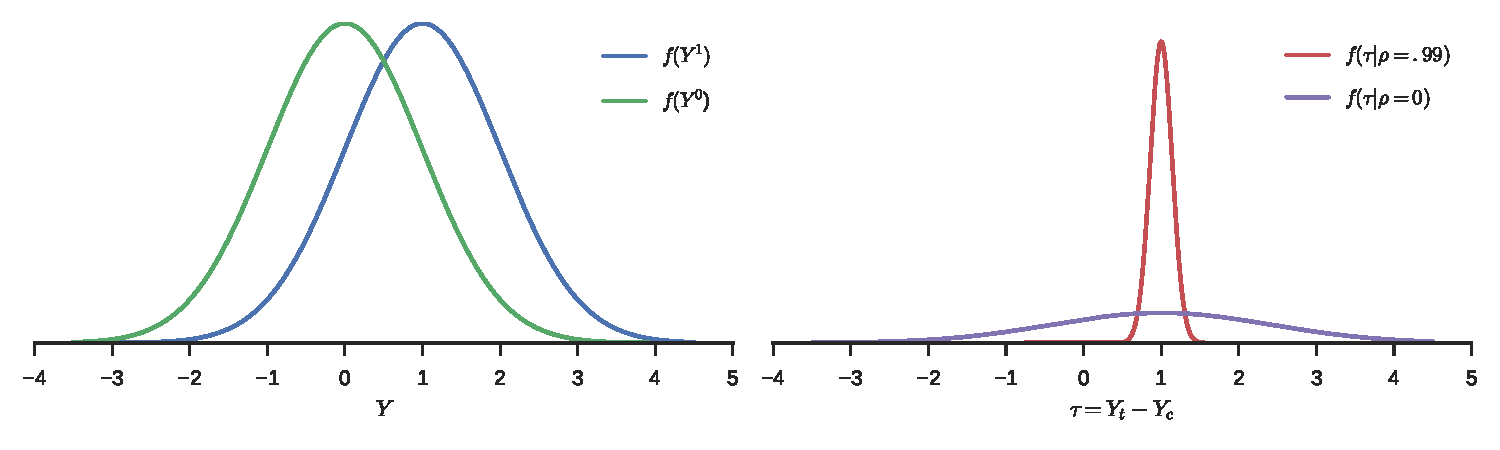
\includegraphics[scale=.6]{figures/counterfactual_nonidentify.pdf}

Key issue is that we can never observe the joint distribution over $Y_t$ and $Y_c$. As a result, the variance of $\tau$ is not identifiable, even from experimental data. It seems on the face of it that $\tau$ is relevent to our decision making. If the example above, if $\rho = 1$ then almost everyone benifits slightly from the treatment. However if $\rho=0$, there is a wide range, with some people benifiting a lot and others suffering significant harm.  

Can these issues be resolved? If so, how? 

- note that we can bound this counterfactual distribution based on the variance of the observed interventional distributions. If the variance of XXX is small then this may not be an issue. 

- does it actually make sense to make a decison on the basis of this counterfactual that is a function of something we could never observe. I

- part of the problem may be due to the deteminisitic way we have phrased individual treatment effects. 

Can these issues be resolved by considering personalized causal effects as random variables and avoiding counterfactuals?

A range of similar issues can arise in counterfactuals \ref{XXXX}. 
- What assumptions are required for the kind of counterfactual analysis like X would have been higher had B ...?
- briefly discuss the different flavours of counterfactual questions here. 

One way of looking at counterfactuals is as a natural language short hand for describing highly specific interventions like those denoted by the do-notation. Rather than taking about the distribution of Y given we intervene to set $X=x$ and hold everything else about the system constant we just say what would the distribution of $Y$ be had $X$ been $X$. This is certainly convienient, if rather impressise. 


\subsection*{Comparing and unifying the models}

Remarkably for models developed relatively independently in fields with very different approaches and problems, the models we have discussed can be nicely unified for interventional queries (those that can be expressed with the do-notation). This makes it straighforward to combine key results and algorithms developed within any of these frameworks. For example, draw a graphical network to determine if a problem is identifiable and which variables should be adjusted for to obtain an unbiased causal estimate. Then use propensity scores \ref{} estimate the effect. If non-parametric assumptions are insufficient for identification or lead to overly large uncertainties, you can specify additional assumptions by phrasing your model in terms of structural equations. 

If the network for a structural equation model is acyclic, that is if starting from any node and following edges in the direction of the arrows you cannot return to the starting point, then it implies a recursive factorization of the joint distribution over its variables. In other words, the network is a causal Bayesian network. All of the results that apply to causal Bayesian networks also apply to acyclic structural equation models.  Taking an action that sets a variable to a specific value equates to replacing the equation for that variable with a constant. This corresponds to dropping a term in the factorization and the truncated product formula (equation \ref{eq:truncatedproduct}). Thus, the interventional query $P(Y|do(X))$ is identical in these two frameworks. We can also connect this to counterfactuals via:

\begin{equation}
\begin{aligned}
&Y^{0} \equiv P(Y|do(X=0)) \\
&Y^{1} \equiv P(Y|do(X=1))
\end{aligned}
\end{equation}

The assumption $\epsilon_{X} \ci \epsilon_{Y}$, stated for our structural equation model, translates to $X \ci (Y^{0},Y^{1})$ in the language of counterfactuals. When discussing the counterfactual model, we actually made the slightly weaker assumption:

\begin{equation}
\label{eq:weakignore}
X \ci Y^{0} \text{ and } X \ci Y^{1}
\end{equation}

It is possible to relax the independence of errors assumption we made for SEMs slightly to correspond exactly the form of equation (\ref{eq:weakignore}) without losing any of the power provided by d-separation and graphical identification rules \cite{Richardson2013}. To determine if and how an interventional query can be non-parametrically identified, it is equivalent to specify assumptions graphically in terms of functional models or bayesian networks or as conditional independence statements involving counterfactual variables (ignorability assumptions). By non-parametrically, I mean that we are not making any assumptions about the form of the relationships between variables. Models that are not non-parametrically identifiable can still be identified given assumptions about the distributions of variables and the functional relationship between them, for example, that the functions are linear or that the noise is additive \cite{Peters2014}. This form of assumption fits extremely naturally into the structural equation framework. 


However we can also pose causal queries that are not interventional and cannot be phrased in terms of the do-notation. The patients in our drug treatment example could be broken down into four groups. \todo{point out objections to doing this}. The first group will recover whether or not they receive treatment, the second group will recover if treated but not on the placebo, the third group will recover on the placebo and not if treated, and the last group will not recover on treatment or placebo. Unfortunately, we don't know which group each person belongs to. Drawing this up as a table:

\begin{tabular}{c|c|c|c}
group & placebo & treatment & probability of group\\
\hline
1 & die & die & $\alpha=P(Y^{0}=0,Y^{1}=0)$\\
2 & die & recover & $\beta=P(Y^{0}=0,Y^{1}=1)$\\
3 & recover & die & $\gamma=P(Y^{0}=1,Y^{1}=0)$\\
4 & recover & recover & $\delta=P(Y^{0}=1,Y^{1}=1)$\\
\end{tabular}

The queries we have been asking thus far are about $P(Y^{0}=1) = \gamma + \delta$ and $P(Y^{1}=1) = \beta + \delta$, but suppose we asked the question; what is the probability that this patient, who was not treated and died, would have recovered if they had been treated? We know they are in either group 1 or 2 since they died without treatment, so the answer is $\frac{\beta}{\alpha+\beta}$. Can we estimate the $\alpha, \beta, \gamma, \delta$ or in other words, identify the joint distribution over the counterfactuals $P(Y^{0},Y^{1})$ given the interventional distributions, $P(Y^{0})$ and $P(Y^{1})$? The answer is no, putting our constraints and unknowns in matrix form:

\begin{equation}
\left(
\begin{array}{cccc}
0&0&1&1\\
1&1&0&0\\
0&1&0&1\\
1&0&1&0\\
1&1&1&1\\
\end{array}
\right)
\left(
\begin{array}{c}
\alpha\\
\beta\\
\gamma\\
\delta\\
\end{array}
\right)= 
\left(
\begin{array}{c}
P(Y^{0})\\
1-P(Y^{0})\\
P(Y^{1})\\
1-P(Y^{1})\\
1\\
\end{array}
\right)
\implies
\left(
\begin{array}{c}
\alpha\\
\beta\\
\gamma\\
\delta\\
\end{array}
\right)=
\left(
\begin{array}{c}
1-P(Y^{0})-P(Y^{1})+\delta\\
P(Y^{1})-\delta\\
P(Y^{0})-\delta\\
\delta\\
\end{array}
\right)
\end{equation}
The value of $\delta$ is not determined so the query is not identifiable. However we do get bounds on the terms. Since probabilities cannot be negative, $P(Y{1})-P(Y^{0})-1 \leq \delta \leq min(P(Y^{1}),P(Y^{0})$. Note, if we made the additional assumption $\gamma=0$; that the drug did not cause anyone to die who would otherwise have survived, then we can determine the joint distribution over counterfactuals. Alternatively, if we could assume that after treatment people returned to their initial state after some period of time, (say we were testing a drug for acne) then we could run a crossover study to determine the joint distribution. In a crossover study, the participants are randomly assigned to treatment and placebo, results are measured and then the groups are swapped. The scientific and philosophical validity of counterfactual queries remains under question \cite{Dawid2000,Dawid2014}, however they are nonetheless widely posed in the form of attribution of causal effects to different pathways and mediation \cite{Pearl2014,Imai2010a,VanderWeele2011}. 

There are differences between the models we have considered when it comes to counterfactual queries. Counterfactuals are not defined in causal Bayesian networks, as they only encode information on the interventional distribution over variables.  Counterfactuals can be defined in terms of structural equation models \cite{Pearl2000} but there are subtle differences depending on the form of assumptions made. Structural equation models with independent errors allows the identification of quantities in mediation studies, which are not identifiable with the weak ignorability assumptions and cannot be tested experimentally \cite{Richardson2013}.  

In practice, differences in focus and approach across different fields eclipse these actual differences in the models. The work on causal graphical models \cite{Pearl2000,Sprites} focuses on non-parametric estimation in the population limit and rigorous theoretical foundations. The Neyman-Rubin framework builds on our understanding of randomized experiment and generalizes to quasi-exeperimental and observational settings, with a particular focus on non-random assignment to treatment. This research emphasises estimating average causal effects and provides practical methods for estimation, in particular, propensity scores; a method to control for multiple variables in high dimensional settings with finite data \cite{Rosenbaum1983}. In economics, inferring causal effects from non-experimental data so as to support policy decisions is central to the field. Economists are often interested in broader measures of the distribution of causal effects than the mean and make extensive use of structural equation models, generally with strong parametric assumptions \cite{Heckman2008}. In addition, the parametric structural equation models favoured in economics can be extended to analyse cyclic (otherwise referred to as non-recursive) models. 


\subsubsection{A translator from graphical independence to counter factual statements}

\subsubsection*{More terminology}
With the graphical framework in place, it is useful to define some key terminology used in describing causal models in terms of the graph structure they refer to.

\begin{enumerate}
\item confounding
\item exogenous
\item endogenous
\item nuisance variables
\end{enumerate} 

\subsection*{What does a causal model give us? Resolving Simpson's paradox}

We will now demonstrate how we can use our new notation and frameworks for causal inference to resolve a facinating paradox. \todo{ insert some history of simpson's paradox here.}

Suppose a doctor has two treatments, A and B, which she offers to patients for blood preasure control. She keeps track of which medication her patients choose and whether or not the treatment is successful. She obtains the following results:

\todo{insert data table with success by treatment}

It seems that drug A is performing better. However, having read the latest liturature that medication effectiveness may differ between men and women, she decides to check how each drug performed by gender and obtained the following data.

\todo{innsert table}

Once the data is broken down by gender, it appears that treament B is better for both men \emph{and} women. This is the paradox. If the doctor were unaware of the gender, it seems that she should advise treatment A. But as soon as the patient walks though the door  then she should offer treatment B, regardless of which gender the patient turns out to be. How does causaul modelling reslove this paradox? Let's represent the treatment presribed by the variable $T$, the gender of the patient by $Z$ and wheter or not the treatment was successful by $Y$. The key to resolving the paradox is that the doctor really cares about the interventional distribution $P{Y|do(T)}$, not the standard conditional distributions $P{Y|T}$. The results from table XXX shows that $\P{Y|T=A}$ is higher than $\P{Y|T=B}$. If she has to suggest a treatment for a patient without knowing their gender, she should choose the treatment for which $P{Y|do(T)}$ is highest not $P{Y|T}$. If she knows thier gender then she should otimise to $P{Y|do(T),Z}$. 

The causal network for this problem is shown below. In this example, women are more likely to choose treatment $A$ and also more likely to recover regardless of what treatment they recive than men. This is what makes treatment $A$ appear better if you look at the conditional distribution. The fact that a patient took treatment $A$ tells you that they are more likely to be female. In the terminology defined in section \ref{}, gender is a confounding variable and we must adjust for it to obtain unbiased estimates of the causal effect of the treatment. As we saw from the examples in chapter \ref{XXX}. Determining when you really care about the interventional as opposed to the conditional distribution is a sublte but very important question that is frequently overlooked. 


\chapter*{Two key questions (5000 words)}

We can rougly categorize the problems studied within causal inference into two groups, causal effect estimation and causal discovery. In causal effect estimation we assume (at least implicitly) that key aspects of the causal graph are known. The goal is then to estimate the causal effect of some action or range of actions. WHERE DOES MEDIATION FIT IN? THIS IS ALREADY HUGE, and is central to 1000 of papers published each year. Causal discovery aims to leverage much broader assumptions to learn the stucture of causal graph from data. THIS IS THE AUTOMATION OF SCIENCE.

 
\section*{Causal effect estimation} 

Causal effect estimation addresses the problem where we assume the key structure of the graph is known. That is, we assume that we have at a minimum:

\begin{itemize}
\item the target/outcome variable we care about
\item the focus/treatment variables on which we are considering intervetions
\item any variables which act to confound two or more of the variables we have included.
\end{itemize}

Some of these variables my be latent or unobserved, in that we do not have measurements for them in the available data. However, their position in the network is assumed to be known. For example if we were trying to estimate ...

Causal effect estimation is one of the most frequently applied methodolgoies within applied sciences. It implicit in millions of studies accross medicine, business, economics and social sciences. Almost everytime someone runs a regression model the key quantity of interest is a causal effect. Given how it underlies so much of our scientific progress, there is a enormous potential in properly understanding when we can draw causal conclusions, exactly what assumptions are required to do so and how we can best levereage those assumptions to infere as much information as we can from our data. 

\subsection*{The do calculus}
Once we have drawn the causal network for our problem, how can we use that to map information from the observational setting? 

The do calculus arises from d-seperation. 

How do we take our causal frameworks and use them to map information from the observational to interventional settings?

\subsection*{Identifiability}
A natural question to ask is, given the level of assumptions we have made about the graph, is it possible to estimate a causal effect from observational data? This is the identifiablity problem. Identifiability is an asymptopic property of the graph. It asks if we can obtain an unbiased point estimate for the causal effect of interest in the infinite data limit. A problem is non-parametrically identifaible if it is identifiable without any additional assumptions on the functional form of the dependencies between variables in the graph. 

The question of non-parametric identifiability is solved! The do calculus is complete. A problem is identifiable if and only if the interventional distribution of interest can be transformed into term containing only observataional quantities via repeated application of the do calculus. 

There is an algorithm \cite{Shpitser2012} based on these properties that, for a given network and interventional (do-type) query, can:

a) determine if the query can be translated into an expression involving only distributions over observed variables. In other words, determine if the query is identifiable given the assumptions encoded by the network

b) if it is identiable, return the required expression  

\todo{insert link to working javascript version}

There are many interesting questions relating to identifiability that remain open. What is the minimal (by some metric) additional information that would be required to make a non-identifiable qurey identifiable? What if we assume various restrictions on the functional form of the relationships between the variables? Clearly  . A complete algorithm for the problem of linear identifiability is yet to be found, despite a rich body of work going back to at least ??? \ref{}

Is identifiablity a good question to ask? It seems natural to see if a problem can be solved with infinite data before we try to see how well we can do it with finite data. However, we should not give up on non-identifiable problems. We may still be able to achive useful bounds on causal effects with finite data even if point estimation is not possible. From that perspective we should be cautious about dividing problems into identifiable and not identifiable. 

How do we tackle a problem that is not identifiable. We could look for bounds or we could make additional assumptions (or both). 

\subsection*{Estimation}
\subsection*{Defining causal effects} Summarising the difference between two distributions. There is no one answer. \cite{Janzing2013}

\cite{Imbens2004} Review of non-parametric estimation
\cite{causal estimation is covariate shift}
\paragraph*{How well do we actually do with finite datasets?}

\paragraph*{When is regression causal?}
A regression equation is causal if, when we represent the equations as a bayesian causal model or structural equation model, we claim the arrows are causal AND if the variables we include in the regression form a valid back door adjustment set. 

\subsection*{Non identifiable queries}

\subsubsection*{Parametric assumptions}
eg linearity

\subsubsection*{Bounds}
\paragraph{Instrumental variables are an example}

Put in the picture of an instrumental variable.

Instrumental variables are one of the key approaches used to estimate causal effects within economics and the social sciences. However, the setting they are associated with is non-identifiable. How is it that they are so useful nonetheless? Tight bounds may be just as good as what could be achieved in the identifiable setting, given finite data. 

\section*{Causal Discovery}
We now move to the much more general problem of learning a causal graph from observational data. Amazingly, it is possible to infer some aspects of causal structure with very general assumptions. The set of conditional independences in a non-experimental data set indicates some causal structures are more likely than others. In addition, there are subtle asymmetries in the relationship between the joint distribution of cause and effect and the distributions of cause given effect and effect given cause. These clues are the key to causal discovery algorithms, which attempt to learn causal structure from non-experimental data. 

 



\paragraph*{You want to learn the graph}
In the causal discovery problem we make much much broader assumptions about the structure of the graph. Ie that it is acyclic. and may or may not have latent variables. We do not assume the existance or directions of any links between the variables.

What's more, we wish to do this from non-experimental data (although there is also work on infering causal structure from experimental data) REFERENCES and it would be natural to connect the two (ANY REFERENCES THERE?).

This is a much grander goal than causal inference and arguably, if acheived would equate to the automation of scientific discovery. 
\paragraph*{Equates to the aim of automating scientific discovery}
\paragraph*{Increadibly hard}
It it is amazing that anything can be done here.
\paragraph*{Methods can also be divided into contraint based and search and score}
\subsection*{Discovery with Conditional independence}
If variables are (conditionally) independent they are unlikely to be directly causally linked. 
\subsection*{Discovery with Functional Models}
\subsection*{Granger causality}

In previous sections we discussed when assumptions about the structure of the variables in a specific problem is sufficient to identify a causal effect. This approach relies on having enough prior knowledge or theory about the problem to allow you to, at least partially, specify the causal network. In this section, we consider the much harder problem of causal inference where you need to learn the network. Causal inference might seem impossible without specific assumptions about the structure of the variables involved but, amazingly, some aspects of causal structure can be determined from much more general assumptions.  

In this section we consider variants of the following problem: Assume there is some acyclic causal network $G$ that generated the distribution $P(\boldsymbol{V})$ from which our data has been sampled. Our goal is to recover the network from this data. 

What can we look for in the distribution that could give us clues as to the structure of the network? 

\subsection{Causal discovery with conditional independence tests}
One general approach is to look for clues about the structure of the network in the conditional independence relations in the distribution. We know, (section \ref{sec:dsep}), if $Z$ d-separates $X$ and $Y$ in $G$ then $(X \ci Y|Z)$ in $P$ . However, we want to work in the other direction, from conditional independence in the distribution to the structure of the network. This requires that we assume the reverse condition:$(X \ci Y|Z)$ in $P$ must imply $Z$ d-separates $X$ and $Y$ in $G$. This assumption, commonly referred to as  \textbf{\textit{faithfulness}}, says there are no additional independence relations that are satisfied in $P$ but not in all distributions $\boldsymbol{P'}$ that are compatible with $G$. Stating that $P$ is faithful to $G$ is equivalent to $G$ is a \textbf{\textit{perfect map}} for $P$.

Faithfulness is an assumption. It does not always hold and we cannot verify it from the observational data we wish to use for causal inference. However, most distributions generated by a causal bayesian network will be faithful to that network. For faithfulness to be violated, different causal effects must exactly balance one-another out. For example, consider a simple binary variable model of chocolate consumption, income and obesity (figure). If the coefficients in the conditional probability tables are just right then the direct effect of chocolate on obesity will exactly balance the indirect effect through income and obesity will appear independent of chocolate consumption. However, this independence is not stable. It would disappear under a small perturbation to any of the parameters.  

Given the faithfulness assumption, our causal discovery problem reduces to finding the set of bayesian networks that have exactly the dependency structure as we observe in $P$. This set can also be referred to as the markov equivalence class compatible with $P$.

\subsubsection{Without hidden common causes}
The strong assumption that there are no hidden variables that cause two or more variables in $\boldsymbol{V}$ significantly reduces the 'search space' of bayesian networks we must consider. 

We will begin with a brute force algorithm (described as the SGS algorithm in \cite{Sprites} and IC algorithm in \cite{Pearl2000}). While it is impractical for all but the smallest of networks, it demonstrates key concepts that also underlie the more useful and complex algorithms we will discuss later. 

\begin{table}[H]
 \begin{tabularx}{\textwidth}{X}
 \hline
\rule{0pt}{2.5ex} 
 \textbf{The SGS (or IC) Algorithm}\\
 \hline
 \rule{0pt}{2.5ex}
\textbf{Input:} A distribution $P$, over variables $\boldsymbol{V}$, that was generated by and is faithful to an (unknown) bayesian network $G$\\
\textbf{Output:} A partially directed network that represents the markov equivelence class of $G$\\
 \begin{enumerate}[itemsep=8pt]
  \item Join all pairs of vertices $(a,b) \in \boldsymbol{V}$ with an undirected link to form a complete graph.
  \item For each link $a-b$ search for a set $\boldsymbol{S}_{a,b} \subseteq V \setminus \{a,b\}$ that renders $a$ and $b$ conditionally independent. If such a set (including the empty set) exists then $a$ and $b$ cannot be directly connected in $G$ so delete the link.
  \label{alg:SGSexponential}
  
  \item For all pairs of non-linked variables $(\alpha,\beta)$ with a common neighbour, $c$, if $c \notin \boldsymbol{S}_{\alpha,\beta}$, then $c$ must be a collider in the path $\alpha,c,\beta$ so  add arrows to direct the links $\alpha-c$ and $\beta-c$ towards $c$.
  \label{alg:SGScolliders}  
  \item Recursively try to orient any edges that remain undirected to avoid creating cycles (because they are not there by assumption) and additional colliders (because any colliders were found in step \ref{alg:SGScolliders}).
  \label{alg:SGSfinal}
\end{enumerate}\\
 \hline
\end{tabularx}
\end{table}

The SGS algorithm utilizes the fact that a collider structure (f
igure \ref{fig:dseptripple4}) induces a distinct conditional independence relation. Assuming you have a consistent conditional independence test, it converges to return a partially directed network that represents the Markov equivalence class for the generating causal model. Unfortunately the number of conditional independence tests required for step \ref{alg:SGSexponential} grows exponentially (in the worst case) with the number of variables. Not only that, but for each edge that is in the true network, the algorithm will always tests all other possible subsets of variables. If the assumption that there are no hidden common causes or that the distribution is faithful are violated, step \ref{alg:SGScolliders} of the SGS algorithm can produce double headed arrows.

The PC algorithm \cite{Sprites} modifies step \ref{alg:SGSexponential} of the SGS algorithm to utilize the fact that if two variables $(a,b)$ are conditionally independent given some set, they will also be conditionally independent given a set that contains only variables adjacent to $a$ or $b$. It also checks for low order conditional independence relations before higher order ones. This allows it to exploit any sparsity in the true network, leading to much better average case performance  \cite{Sprites} (although the worst case, where the true network is complete, is still exponential). With finite data, the order in which the links are considered can change the output (unlike for SGS). The effect of wrongly removing a link early on flows through to later conditional independence tests by changing which nodes are considered adjacent.


\begin{table}[H]
 \begin{tabularx}{\textwidth}{X}
 \hline
\rule{0pt}{2.5ex} 
 \textbf{The PC Algorithm}\\
 \hline
 \rule{0pt}{2.5ex}
\textbf{Input:} A distribution $P$, over variables $\boldsymbol{V} = \{V_{1}...V_{k}\}$, that was generated by and is faithful to an (unknown) bayesian network $G$\\
\textbf{Output:} A partially directed network that represents the markov equivelence class of $G$\\
 \begin{enumerate}[itemsep=8pt]
  \item As for SGS
  \item \textbf{for} each link $a-b$:
  \begin{itemize}[label={}]
   \item $n = 0$
   \item $\boldsymbol{A}_{a,b} = \{A_{1}...A_{j}\}$ be the set of nodes adjacent to $a$ and/or $b$
   \item \textbf{while} $a$ and $b$ are connected and $n < j$:
   \item 
    	\begin{itemize}[label={}]
    	\item \textbf{if} any subset of size $n$ of $\boldsymbol{A}$ makes $a$ and $b$ conditionally independent:
    	\item \begin{itemize}[label={}]
    			delete the link
    		  \end{itemize}
    	
    	\item $n = n+1$
    	\end{itemize}
  \end{itemize}   
  \item as for SGS
  \item as for SGS
\end{enumerate}\\
 \hline
\end{tabularx}
\end{table}

The PC algorithm also returns a set of Markov equivalent networks consistent with the distribution. Since we have assumed there are no hidden variables, for any single graph in this set we can calculate causal effects with equation \ref{eq:allvarsobserved}. We can then bound the true causal effect by combining the results for the all the networks. This procedure is the IDA algorithm \cite{Maathuis2009} and has been found to outperform standard regularization techniques at finding causal effects in a high-dimensional yeast gene expression data set \cite{Maathuis2010}. An implementation is available in the R package \cite{Kalisch2012} 


\subsubsection{With hidden variables}
There are an number of difficulties in extending the approach of the last section to deal with the case where there are latent variables. With an unknown number of hidden variables there are an infinity many possible structures to search over. In addition, the space of causal networks is not closed under marginalization. If we have a distribution that $P'(\boldsymbol{O},\boldsymbol{U})$ generated by and is faithful to a network $G$ the distribution $P(\boldsymbol{O})$, that results from marginalizing over $\boldsymbol{U}$, may not be faithful to any bayesian network (see figure \ref{fig:DAGSnotclosed}).

%\begin{figure}
%\centering
%\caption{A distribution faithful to this DAG is not faithful to any DAG over the variables $\{A,B,C,D\}$ after marginalizing over $U$. }
%\label{fig:DAGSnotclosed}
% \begin{tikzpicture}[->,>=stealth',shorten >=1pt,auto,node distance=1cm,  thick,main node/.style={punkt}]
% %nodes
%\node[main node](1){U}; 
%\node[main node, below left = of 1](2){B};
%\node[main node, below right = of 1](3){C};
%\node[main node, above left= of 2](4){A};
%\node[main node, above right = of 3](5){D};
%
% \path[every node/.style={font=\sffamily\small}]
%    (1) edge node {} (2)
%    	edge node {} (3)
%    (4) edge node {} (2)
%    (5) edge node {} (3);
%    	
%\end{tikzpicture}
%\end{figure}
 

The key to constraining the space of possible models is that many latent structures are equivalent (under transforms of the hidden variables). See example figure XXX.

\begin{theorem}
\cite{Verma1993} For every latent structure there is a dependency equivalent structure such that every latent (unobserved) variable is a root node with exactly two children .
\end{theorem}

Since we only care about the causal relationships between observed variables, it is sufficient to search over networks where any hidden variables have no parents and directly cause two of the observed variables. Instead of representing hidden variables explicitly we can capture the necessary independence relations with a more general graphical model that supports bi-directed edges that play the role of a hidden confounding variable. These models, referred to as maximal ancestral graphs (MAGs) are closed under marginalization and conditioning. 

For any DAG with latent (and selection) variables there is a unique MAG \cite{Richardson2002}. This makes it possible to extend the PC algorithm to latent structures, resulting in the FCI algorithm \cite{Sprites}. The logic is very similar. Certain structures are ruled out by being inconstant with the observed conditional independence relations. The output is an equivalence class of MAGs, which can be represented graphically as a partial ancestral graph PAG. Assuming there are no selection variables (see \cite xxx), the PAG can contain four types of link:

\begin{enumerate}
\item $X \rightarrow Y$, meaning $X$ causes $Y$
\item $X \leftrightarrow Y$, meaning there is a latent variable that causes $X$ and $Y$.
\item $X\ {\circ} {\rightarrow}\ Y$, either $X$ causes $Y$ or a latent variable causes both.
\item $X\ {\circ} {-}  {\circ}\ Y$, either $X$ causes $Y$ or $Y$ causes $X$ or a latent variable causes both.
\end{enumerate}

The circles indicate where it is ambiguous if there should be an arrowhead (ie where there is one in some MAGs and not in others in the equivalence class). Counter-intuitively it is sometimes possible to  rule out or confirm the existence of a confounding variable and fully determine the causal type of a link (see examples in figure \ref{fig:FCIExamples}). 

%\begin{figure}
%\centering
%\caption{A distribution faithful to this DAG is not faithful to any DAG over the variables $\{A,B,C,D\}$ after marginalizing over $U$. }
%\label{fig:FCIExamples}
% \begin{subfigure}[t]{0.8\textwidth}
% \begin{tikzpicture}[->,>=stealth',shorten >=1pt,auto,node distance=.7cm,  thick,main node/.style={punkt}]
% %nodes
%\node[main node](1){U}; 
%\node[main node, below left = of 1](2){B};
%\node[main node, below right = of 1](3){C};
%\node[main node, above left= of 2](4){A};
%\node[main node, above right = of 3](5){D};
%
% \path[every node/.style={font=\sffamily\small}]
%    (1) edge node {} (2)
%    	edge node {} (3)
%    (4) edge node {} (2)
%    (5) edge node {} (3);
%    	
%\end{tikzpicture}
% \end{subfigure}
% \begin{subfigure}[t]{0.8\textwidth}
% \begin{tikzpicture}[->,>=stealth',shorten >=1pt,auto,node distance=.7cm,  thick,main node/.style={punkt}]
% %nodes
%
%\node[main node](1){A};
%\node[main node, below right=of 1](2){B};
%\node[main node, right=of 2](3){C};
%\node[main node, above right=of 3](4){D};
%
% \path[every node/.style={font=\sffamily\small}]
%    (1) edge[pil] node {} (2)
%    (2) edge node {} (3)
%    (3) edge node {} (2)
%    (4) edge [pil] node {} (3);    	
%\end{tikzpicture}
%\end{subfigure}
% \begin{subfigure}[t]{0.4\textwidth}
% \begin{tikzpicture}[->,>=stealth',shorten >=1pt,auto,node distance=0.7cm,  thick,main node/.style={punkt}]
% %nodes
%
%\node[main node](1){C};
%\node[main node, above left=of 1](2){A};
%\node[main node, above right=of 1](3){B};
%\node[main node, below=of 1](4){D};
%
% \path[every node/.style={font=\sffamily\small}]
%    (1) edge node {} (4)
%    (2) edge node {} (1)
%    (3) edge node {} (1);    	
%\end{tikzpicture}
%\end{subfigure}
% \begin{subfigure}[t]{0.4\textwidth}
% \begin{tikzpicture}[->,>=stealth',shorten >=1pt,auto,node distance=0.7cm,  thick,main node/.style={punkt}]
% %nodes
%
%\node[main node](1){C};
%\node[main node, above left=of 1](2){A};
%\node[main node, above right=of 1](3){B};
%\node[main node, below=of 1](4){D};
%
% \path[every node/.style={font=\sffamily\small}]
% 	(1) edge node {} (4)
%    (2) edge [pil] node {} (1)
%    (3) edge [pil] node {} (1);    	
%\end{tikzpicture}
%\end{subfigure}
%\end{figure} 

The FCI algorithm can be made complete such that it discovers all aspects of the true causal structure that are identifiable from the conditional independence relations of a distribution over observed variables and the faithfulness assumption \cite{Zhang2008}. More recently \cite{Colombo2012} have proposed the RFCI algorithm, which in some cases returns more ambiguous links than FCI but is substantially faster. \cite{Claassen2013} point out that the problem of learning sparse causal networks from data is not NP-hard and propose the FCI+ algorithm, that requires $O(N^{2(k+2)})$ conditional independence tests, where $k$ is the maximum node degree over the observed variables. 

With latent variables we are not using all the information - so we could go further (to nested markov models and inequalities.) \cite{Richardson2012} \cite{Shipster2014}


These are all constraint based methods ... efficient because they stop early, but also may not be robust to errors early on. 

A comparison of algorithms 

\renewcommand{\arraystretch}{1.5}
\begin{tabular}{| c | c | p{4cm} | c | c | c |}
\hline
  \textbf {Alg.} &\textbf{ Method }& \textbf{Scales (num.vars) }& $\sim $ \textbf {Vars} & \textbf {Latent } & \textbf {Reference} \\
  \hline
  IC/SGS & Constraint based & Exponential & 10 & No & Pearl(2000)/Sprites(2000)\\
  \hline
  PC & Constraint based & Worst case exponential, polynomial for sparse graphs & 5000 & No & Sprites(2000) \\ 
  \hline
  FCI & Constraint based & Worst case exponential, polynomial variant FCI+ for sparse graphs & 30 & Yes & Sprites(2000) \\
  \hline
  RFCI & Constraint based & ? & 500 & Yes & Colombo(2012) \\
  \hline
  GES & Search \& Score  & Worst case exponential & 50 & No & Chickering(2002) \\
  \hline
  MMHC & Hybrid & ? & 5000 & No & Tsamardinos(2006) \\
 \hline
\end{tabular}

\subsubsection{Doing conditional independence tests}
The off-diagonal elements of the standardized inverse of the correlation
matrix are the negatives of the partial correlation coefficients between the corresponding
variables given the remaining variables (see e.g. Whittaker, 1990). Hence in the linear case, the
independence graph can be efficiently constructed by placing an edge between A and B if and
only if the entry in the standardized inverse correlation matrix is non-zero. In the discrete case,
Fung and Crawford (1990) have recently proposed a fast algorithm for constructing an
independence graph from discrete data. We have not tested their procedure as a preprocessor for
the PC algorithm. (COPIED FROM SPRITES)

\cite{Zhang2012} Kernel independence tests

HSIC \cite{Gretton2008}

\subsection{Discovery with functional models}
All of the algorithms we have considered so far return a Markov equivalence class. They cannot distinguish between two models that result in the same set of conditional independence relations. Consider the very simple case where we have only two variables and the only possible causal structures are $X \rightarrow Y$ or $Y \rightarrow X$. These models have the same dependency structure but in one case $P(Y|do(X)) = P(Y|X)$ and in the other $P(Y|do(X)) = P(Y)$. No algorithm relying purely on conditional independence relations can separate these two cases. 

Let us focus only on the two variable case $X \rightarrow Y$ or $Y \rightarrow X$. What possible clues could there be in the distribution $P(X,Y)$ that could indicate which causal model it was generated from. Recall the functional definition of causality (section \ref{sec:SEM}). There are a number of assumptions about the form of the functions that can allow us to identify the causal direction: non-invertible functions, additive noise \ref{}, post-non-linear additive noise 


Linear models with non-gaussian noise \cite{Hoyer2012}

Allow us to make assumptions about the form of the relationships between variables.
With just two variables:

Additive noise, \cite{Hoyer2009}

post-non-linear additive noise \cite{Zhang2008a}, 

causal anti-causal, 

deterministic functions,

IGCI \cite{Janzing2012a}

learning what causality looks like.

If we have a method to solve this case we can solve the more general case (with no hidden variables) Putting things together to learn the full network. 


\subsection{Scoring}



\chapter*{The interventionalist viewpoint (5000 words)}

The previous sections all focus on aspects of the question; how can we estimate the effect of an intervention in a system from data collected prior to taking it. There is an obvious alternative. Instead of trying to infer the outcome of an intervention from passive observations we could just do it and see what happens. There are two key differences between observing a system and explicitly intervening in it. Firstly, when we intervene, we can choose which actions to take and thus get some control over which distributions we learn about. Secondly, if we are explicitly choosing interventions, we have a perfect model of the probability that we select each action given any context, allowing us to control confounding bias. 

\subsection*{The role of randomization}

\paragraph*{The interventionalist viewpoint has devloped from the starting point of randomized controlled experiment}

What is the role of randomization? How do bandits algorithms work despite being only partially randomized? 
What else can you do to improve randomized studies (variance reduction, lower regret).

Figure showing how randomization breaking any confounding links

Randomization does not ensure target and control group are exactly alike. The more features or variables you include, the more likely that there will be a significant difference across at least one variable. But the within group variance also increases, the net effect is that it becomes harder to draw a conclusion but not more biased.

\paragraph*{Limitations of randomization} 

\subsection*{Limitations of experimentation} 

Failure to generalize. Transportability, imperfect compliance. Too many contexts.


\paragraph*{internal validity} Are differences in treatment and control groups down to intervention or the result of bias? 

\paragraph*{external validity} Are the results of the study applicable to the broader population of interest.


\section*{Multi armed bandits}
\paragraph*{Definition} 

\paragraph*{What limitations of randomized experiment does the bandit view address}

\paragraph*{The exploration/exploitation trade-off}

\subsection*{Regret} How do we measure the performance of a bandit algorithm?

%$\simpleregret = \mu^* - \E{\mu_{\hat a^*_T}}.$ 

Expected Regret
\eqn{
R_T(\pi) = \E{max_{i \in [k]} \sum_{t=1}^T{X_{t,i}}} - \E{\sum_{t=1}^T{X_{t,A(t)}}}
}

Psuedo-Regret
\eqn{
R_T(\pi) &= max_{i \in [k]}\E{\sum_{t=1}^T{X_{t,i}}} - \E{\sum_{t=1}^T{X_{t,A(t)}}} \\
&= n\mu_{i^*} - \E{\sum_{t=1}^T{X_{t,A(t)}}}
}

Simple Regret
\eqn{
\mu_{i^*} - \E{\mu_{\hat i^*}}.
}

\subsection*{Adversarial Bandits}
What problem do they solve?


\subsection*{Key approaches and results}
\paragraph*{optimisim in the face of uncertainty}

\subsection*{The need to add structure}
\paragraph*{The regret for a bandit problem grows linearly with the number of (sub-optimal) actions.} This makes problems with large or infinite actions spaces intractible.


\subsection*{Key extensions}

\subsubsection*{Contexual bandits}
\paragraph*{Feature selection} Is it even more important here? How do algorithms degrade as irrelevent features are added? In the supervised vs the RL setting? What would be a fair comparison?

\subsubsection*{Markov decision processes}
\subsubsection*{Dynamic Systems}
\begin{itemize}
\item An explicit model of actions in a partially known system (eg HMM)
\item Feynman-Kac Lemma; Solving a PDE can be converted to a stochastic process
\end{itemize}


\chapter*{Causal Bandits: Unifying the approaches (5000 words)}

\section*{The framework}
A natural way to connect the causal framework with the bandit setting is to model the action space as interventions on variables in a causal directed acyclic graph. Each possible assignment of variables to values is a potential action (or bandit arm), see figure \ref{} for a simple example. In some settings, it makes sense to restrict the action space available to the agent to a subset of all the possible actions, for example only the set of single variable interventions. The reward could be a general function of the action selected and the final state of the graph. However for simplicity, we will consider the reward to be the value of a single specified node minus the cost of the selected action. In this thesis I examine the case where the causal graph is known. We refer to these problems as \emph{causal bandit problems}.  Extending this work to simultaneously learning the casusl graph is discussed in section \ref{XXX}.

\subsubsection*{Definition of casual bandit problem} \todo{make proper definition}
A learner for a casual bandit problem is given the casual model's graph $\mathcal{G}$ and a set of \emph{allowed actions} $\mathcal{A}$.
One variable $Y \in \mathcal{X}$ is designated as the \emph{reward variable} and takes on values in $\{0, 1\}$.


\begin{figure}[h]
\caption{A simple causal graphical model and corresponding complete action space. A and B represent binary variables that can be intervened on and Y represents the reward.}
\label{fig:unify_frameworks}
\centering
\begin{subfigure}[c]{0.3\textwidth}
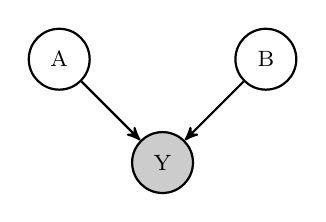
\begin{tikzpicture}[->,shorten >=0pt,shorten <=0pt,node distance=3em,thick,main node/.style={observed}, tg/.style={target}]
\node[main node](1){A};
\node[tg, below right=of 1](2){Y};
\node[main node, above right=of 2](3){B};
\path[]
	(1) edge (2)
	(3) edge (2);
\end{tikzpicture}
\end{subfigure}
\begin{subfigure}[t]{0.4\textwidth}
Actions = \begin{tabular}{|c|}
	\hline
  do(A=0,B=0) \\
  do(A=0,B=1) \\
  do(A=1,B=0) \\
  do(A=1,B=1) \\
  \hline
  do(A=0) \\
  do(A=1) \\
  do(B=0) \\
  do(B=1) \\
  do() \\
  \hline
\end{tabular}
\end{subfigure}
\end{figure} 

The number of actions or arms grows exponentially with the number of variables in the graph,
making it important to use algorithms that leverage the graph structure to reduce the
search space. Modelling a problem as a causal graph only makes sense when rewards are generated stochastically - since causal graphs fundamentally model probability distributions over variables. Thus the connection is to stochastic bandit problems (although adversarial bandits algorithms may be applied to stochastic problems).

We now need to specify the feedback model for the causal bandit problem. What information is available to the decision making agent before and after they select an action? The causal bandit problem takes on characteristics of different bandit settings depending on the assumptions we make about what actions are available to the agent, what variables are obvserved and whether they are observed before or after the action is chosen. 

Enumerate the settings
\begin{enumerate}
\item Bandit feedback: the agent selects an action and then observes only the reward of that action. If feedback is received only on the reward node then the do-calculus can be applied to eliminate some actions immediately, before any experiments are performed and then a standard bandit algorithm can be run on the remaining actions. See figure XXX as an example. 
\item Bandit feedback with side information (context). The agent can view the value of some variables prior to selecting an action. After selecting they observe the reward of the selected node. 
\item Post action feedback:
\end{enumerate}

If we receive feedback on additional nodes, the problem can be more interesting. In addition to being able to eliminate some actions prior to sampling any data as in the previous case, taking one action may give us some information on actions that were not selected. Consider again the model in figure \ref{fig:unify_frameworks}. The causal structure implies: 

\eqn {
P(Y|do(A = 0)) &= P(Y|do(),A = 0) \\
&= P(Y|do(B=0),A=0)P(B=0)+P(Y|do(B=1),A=0)P(B=1) 
}

Thus we gain information about the reward for the action $do(A=0)$ from selecting the action $do()$ or $do(B = b)$ and then observing $A = 0$.  

We only get this form of side information for actions that don't specify the value of every variable, ie those in the bottom half of the table in figure \ref{fig:unify_frameworks}. Since the reward distribution for actions that set a subset of the variables is the result of marginalizing out other variables, they can only be optimal if they have lower cost. So if the cost of all actions is constant (no matter how many variables must be set), then the problem has the same characteristics as if only the reward node were observable.

If the information on the value of additional nodes is available prior to selecting an action the problem resembles a contextual bandit. For example if we observe $A = 0$ then, in deciding between the actions $do(B=0)$ and $do(B=1)$, we would want information on $P(Y|A=0,B=0)$ and $P(Y|A=0,B=1)$.  Note, side information can still arise if we learn the value of some variables prior to selecting an action and some afterwards. 

Although we will focus on the intervene-then-observe ordering of events within each round, other scenarios are possible. If the non-intervened variables are observed before an intervention is selected our framework reduces to stochastic contextual bandits, which are already reasonably well understood~\citep{Agarwal2014}. Even if no observations are made during the rounds, the causal model may still allow offline pruning of the set of allowable interventions thereby reducing the complexity.


\section*{Related work}
\begin{enumerate}
\item leaning from log data
\item bandits with imperfect compliance
\item rigged casino paper
\end{enumerate}

\begin{figure}[h]
\caption{Example causal graph (based on \cite{Koller2009}) where the outcome of interest (reward) is cholesterol level . The do-calculus can be applied to eliminate some actions immediately without the need to do any experiments. For example, no actions involving 'Test Result' need to be considered and interventions on 'Diet' do not need to be considered in conjunction with any other variables.}
\label{fig:cholesterol_graph}
\centering
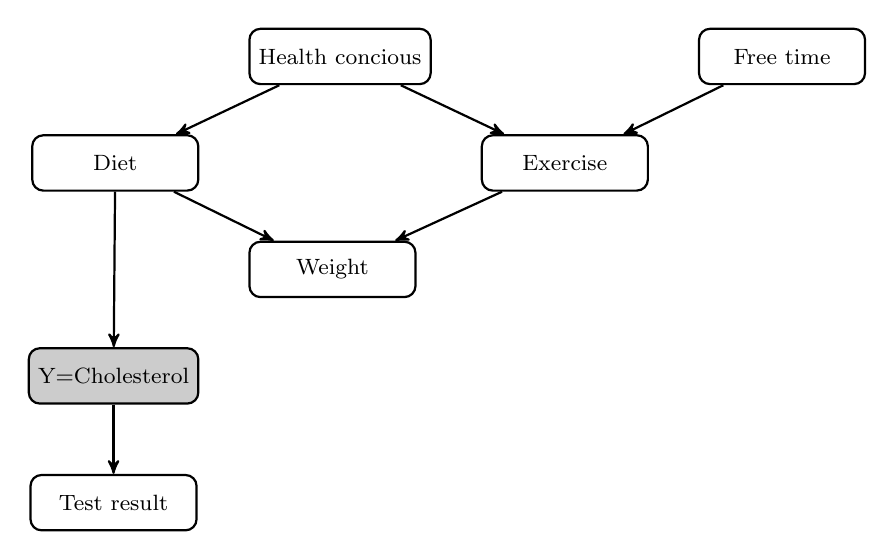
\begin{tikzpicture}[->,shorten >=0pt,shorten <=0pt,node distance=2.5em,thick,node/.style={observedrect},tg/.style={targetrect}]
\node[node](1){Health concious};
\node[node, below left=of 1](2){Diet};
\node[node, below right=of 1](3){Exercise};
\node[node, below right=of 2](4){Weight};
\node[tg,below left=of 4](5){Y=Cholesterol};
\node[node, below =of 5](6){Test result};
\node[node, above right=of 3](7){Free time};
\path[]
	(1) edge (2) edge (3)
	(2) edge (4) edge (5)
	(3) edge (4)
	(5) edge (6)
	(7) edge (3);
\end{tikzpicture}
\end{figure}


\section*{Causal bandits with post action feedback}
WHY THIS PROBLEM. This work was presented at NIPS 2016 \ref{}.
\todo{add relevent stuff from introduction section}

\subsection*{Notation}

We will assume each variable only takes on a finite number of distinct values. (The path to relaxing this assumption would be through leverging the work on continuous armed bandits). 

The \emph{parents} of a variable $X_i$, denoted $\parents{X_i}$, is the set of all variables $X_j$ such that there is an edge from $X_j$ to $X_i$ in $\mathcal{G}$.

An \emph{intervention or action (of size $n$)}, denoted $do(\vec{X}=\vec{x})$, assigns the values $\vec{x}=\{x_1, \ldots, x_n\}$ to the corresponding variables $\vec{X}=\{X_1, \ldots, X_n\} \subset \mathcal{X}$ with the empty intervention (where no variable is set) denoted $do()$.


We denote the expected reward for the action $a = do(\vec{X} = \vec{x})$ by $\mu_{a} := \E{Y | do(\vec{X} = \vec{x})}$ and 
the optimal expected reward by $\mu^* := \max_{a\in\actions} \mu_{a}$. 


\subsection*{Definition of causal bandit game with post-action feedback}
\todo{ re-read and incorporate response from reviewer feedback for NIPS}

The causal bandit game proceeds over $T$ rounds.
In round $t$, the learner \emph{intervenes} by choosing $a_t = do(\vec{X}_t = \vec{x}_t) \in \mathcal{A}$ based on previous observations. 
It then \emph{observes} sampled values for all non-intervened variables $\vec{X}^c_t$ drawn from $\P{\vec{X}^c_t | do(\vec{X}_t = \vec{x}_t)}$, 
including the \emph{reward} $Y_t \in \{0,1\}$. 
After $T$ observations the learner outputs an estimate of the optimal action $\hat a^*_T \in \actions$ based on its prior observations.

The objective of the learner is to minimise the simple regret $\simpleregret = \mu^* - \E{\mu_{\hat a^*_T}}.$ This is sometimes refered to as a ``pure exploration''~\citep{Bubeck2009a} or ``best-arm identification'' problem~\citep{Gabillon2012a} and is most appropriate when, as in drug and policy testing, the learner has a fixed experimental budget after which its policy will be fixed indefinitely. 

We note that classical $K$-armed stochastic bandit problem can be recovered in our framework by considering a simple causal model with one edge connecting a single variable $X$ that can take on $K$ values to a reward variable $Y \in \set{0,1}$ where $\P{Y = 1|X} = r(X)$ for some arbitrary but unknown, real-valued function $r$. The set of allowed actions in this case is $\mathcal{A} = \{ do(X = k) \colon k \in \{1, \ldots, K\}\}$. Conversely, any causal bandit problem can be reduced to a classical stochastic $|\mathcal{A}|$-armed bandit problem by treating each possible intervention as an independent arm and ignoring all sampled values for the observed variables except for the reward. Intuitively though, one would expect to perform better by making use of the extra structure and observations.


\subsection*{The parallel bandit problem}

In this section we propose and analyse an algorithm for achieving the optimal regret in a natural special case of the causal bandit problem which we call the {\it parallel bandit}.
It is simple enough to admit a thorough analysis but rich enough to model the type of problem discussed in \ref{XXX}, including the farming example. It also suffices to witness the regret gap between algorithms that make use of causal models and those which do not.

The causal model for this class of problems has $N$ binary variables $\{ X_1, \ldots, X_N \}$ where each $X_i \in \{0,1\}$ are independent causes of a reward variable $Y \in \set{0,1}$, as shown in Figure~\ref{fig:parallel}. All variables are observable and the set of allowable actions are all size 0 and size 1 interventions: $\mathcal{A} = \set{do()} \cup \set{ do(X_i = j) \colon 1 \leq i \leq N \text{ and } j \in \set{0,1}}$

In the farming example from the introduction, $X_1$ might represent temperature (\eg, $X_1=0$ for low and $X_1=1$ for high). The interventions $do(X_1 = 0)$ and $do(X_1 = 1)$ indicate the use of shades or heat lamps to keep the temperature low or high, respectively.

\begin{figure}
    \begin{subfigure}[b]{0.34\textwidth}
	\centering    
          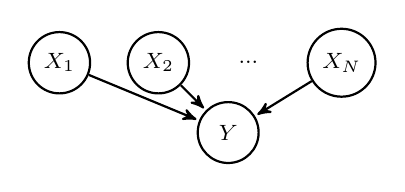
\begin{tikzpicture}[->,>=stealth',shorten >=1pt,auto,node distance=.45cm,
  thick,main node/.style={observed}, hidden/.style={empty},background rectangle/.style={fill=olive!45}]
%every node/.style={scale=0.6}
 %nodes
\node[main node](1){$X_{1}$};
\node[main node, right=of 1](2){$X_{2}$};
\node[hidden, right=of 2](3){$...$};
\node[main node, right=of 3](4){$X_{N}$};
\node[main node, below right=of 2](5){$Y$};
 \path[every node/.style={font=\tiny}]
    (1) edge (5)
    	(2) edge (5)
    (4) edge (5);
\end{tikzpicture}
        \caption{Parallel graph}
        \label{fig:parallel}
    \end{subfigure}
    \begin{subfigure}[b]{0.2\textwidth}
    \centering
        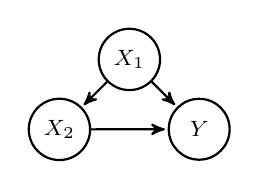
\begin{tikzpicture}[->,>=stealth',shorten >=1pt,auto,node distance=.45cm,
  thick,main node/.style={observed}, hidden/.style={empty},background rectangle/.style={fill=olive!45}]
\node[main node](1){$X_1$};
\node[main node, below left=of 1](2){$X_2$};
\node[main node, below right=of 1](4){$Y$};
 \path[every node/.style={font=\tiny}]
    (1) edge (2)
    (1) edge (4)
    (2) edge (4);
\end{tikzpicture}
        \caption{Confounded graph}
        \label{fig:causalStructure_confounded}
    \end{subfigure}
    \begin{subfigure}[b]{0.4\textwidth}
    \centering
         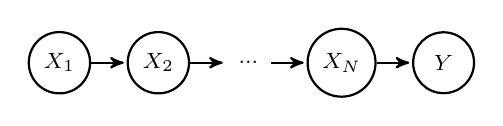
\begin{tikzpicture}[->,>=stealth',shorten >=1pt,auto,node distance=.45cm,
  thick,main node/.style={observed}, hidden/.style={empty},background rectangle/.style={fill=olive!45}]
\node[main node](1){$X_{1}$};
\node[main node, right=of 1](2){$X_{2}$};
\node[hidden, right=of 2](3){$...$};
\node[main node, right=of 3](4){$X_{N}$};
\node[main node, right=of 4](5){$Y$};
 \path[every node/.style={font=\tiny}]
    (1) edge (2)
  	(2) edge (3)
    (3) edge (4)
    (4) edge (5);
\end{tikzpicture}
        \caption{Chain graph}
        \label{fig:causalchain}
    \end{subfigure}
    \caption{Causal Models}\label{fig:causalmodels}
    \vspace{-.5cm}
\end{figure}


In each round the learner either purely observes by selecting $do()$ or sets the value of a single variable. The remaining variables are simultaneously set by independently biased coin flips. The value of all variables are then used to determine the distribution of rewards for that round. Formally, when not intervened upon we assume that each $X_i \sim \bernoulli(q_i)$ where $\vec{q} = (q_1, \ldots, q_N) \in [0,1]^N$ so that $q_i = \P{X_i = 1}$.

The value of the reward variable is distributed as $\P{Y = 1|\vec{X}} = r(\vec{X})$ where 
$r : \{0,1\}^N \to [0,1]$ is an arbitrary, fixed, and unknown function. 
In the farming example, this choice of $Y$ models the success or failure of a seasons crop, 
which depends stochastically on the various environment variables.


\paragraph{The Parallel Bandit Algorithm}
%\label{sub:par-bandit-alg}
The algorithm operates as follows. For the first $T/2$ rounds it chooses $do()$ to collect observational data. As the only link from each $X_1,\ldots,X_N$ to $Y$ is a direct, causal one, $\P{Y|do(X_i=j)}=\P{Y|X_i=j}$. Thus we can create good estimators for the returns of the actions $do(X_i = j)$ for which $\P{X_i = j}$ is large. The actions for which $\P{X_i = j}$ is small may not be observed (often) so  estimates of their returns could be poor. To address this, the remaining $T/2$ rounds are evenly split to estimate the rewards for these infrequently observed actions. The difficulty of the problem depends on $\vec{q}$ and, in particular, how many of the variables are unbalanced (\ie, small $q_i$ or $(1-q_i)$). For $\tau \in [2...N]$ let $I_\tau = \set{ i : \min\set{q_i, 1-q_i} < \frac{1}{\tau}}$. Define

\eq{
\label{eq:m-simple}
m(\vec{q}) = \min \set{ \tau : |I_{\tau}| \leq \tau}\,.
}


\begin{algorithm}[H]
\caption{Parallel Bandit Algorithm}\label{alg:simple}
\begin{algorithmic}[1]
\STATE {\bf Input:} Total rounds $T$ and $N$.
\FOR{$t \in 1,\ldots,T / 2$}
\STATE Perform empty intervention $do()$
\STATE Observe $\vec{X}_t$ and $Y_t$
\ENDFOR
\FOR{$a = do(X_i = x) \in \actions$}
\STATE Count times $X_i = x$ seen: $T_a = \sum_{t=1}^{T/2} \ind{X_{t,i} = x}$
\STATE Estimate reward: $\hat{\mu}_a = \frac{1}{T_a} \sum_{t=1}^{T/2} \ind{X_{t,i} = x} Y_t$ \\[0.2cm]
\STATE Estimate probabilities: $\hat{p}_a = \frac{2 T_a}{T}$,\,\, $\hat q_i = \hat p_{do(X_i = 1)}$
\ENDFOR
\STATE Compute $\hat{m} = m(\vec{\hat q})$ and $A = \set{a \in \actions \colon \hat{p}_a \leq \frac{1}{\hat m}}$.
\STATE Let $T_A := \frac{T}{2 |A|}$ be times to sample each $a\in A$.
\FOR{$a = do(X_i = x) \in A$}
\FOR{$t \in 1,\ldots,T_A$}
\STATE Intervene with $a$ and observe $Y_t$
\ENDFOR
\STATE Re-estimate $\hat{\mu}_a = \frac{1}{T_A} \sum_{t=1}^{T_A} Y_t$
\ENDFOR
\RETURN estimated optimal $\hat{a}^*_T \in \argmax_{a\in\actions} \hat{\mu}_a$
\end{algorithmic}
\end{algorithm}

$I_\tau$ is the set of variables considered unbalanced and we tune $\tau$ to trade off identifying the low probability actions against not having too many of them, so as to minimize the worst-case simple regret. When $\vec{q} = (\frac{1}{2}, \ldots, \frac{1}{2})$ we have $m(\vec{q}) = 2$ and when $\vec{q} = (0, \ldots, 0)$ we have $m(\vec{q}) = N$. We do not assume that $\vec{q}$ is known, thus Algorithm \ref{alg:simple} also utilizes the samples captured during the observational phase to estimate $m(\vec{q})$. Although very simple, the following two theorems show that this algorithm is effectively optimal.


\begin{theorem}\label{thm:uq-simple}
Algorithm \ref{alg:simple} satisfies
\eq{
\simpleregret \in \bigo{\sqrt{\frac{m(\vec{q})}{T}\log\left(\frac{NT}{m(\vec{q})}\right)}}\,.
}
\end{theorem}


\begin{theorem}\label{thm:lower}
For all strategies and $T$, $\vec{q}$, there exist rewards such that
$\displaystyle \simpleregret 
\in \Omega\left(\sqrt{\frac{m(\vec{q})}{T}}\right)$.
\end{theorem}


The proofs of Theorems \ref{thm:uq-simple} and \ref{thm:lower} may be found in Sections \ref{sec:thm:uq-simple} and \ref{sec:thm:lower} respectively.

The proofs of Theorems \ref{thm:uq-simple} and \ref{thm:lower} follow by carefully analysing the concentration
of $\hat p_a$ and $\hat m$ about their true values and may be found in the supplementary material.

%We prove a lower bound on the simple regret that matches up to logarithmic factors the upper bound given in Theorem \ref{thm:uq-simple}. 
By utilizing knowledge of the causal structure, Algorithm \ref{alg:simple} effectively only has to explore the $m(\vec{q})$ 'difficult' actions. Standard multi-armed bandit algorithms must explore all $2N$ actions and thus achieve regret  $\smash{\Omega(\sqrt{N/T})}$. Since $m$ is typically much smaller than $N$, the new algorithm can significantly outperform classical bandit algorithms in this setting. In practice, you would combine the data from both phases to estimate rewards for the low probability actions. We do not do so here as it slightly complicates the proofs and does not improve the worst case regret.

\subsection*{General graphs}
We now consider the more general problem where the graph structure is known, but arbitrary. For general graphs, $\P{Y|X_i=j} \neq \P{Y|do(X_i=j)}$ (correlation is not causation). However, if all the variables are observable, any causal distribution $\P{X_1...X_N|do(X_i=j)}$ can be expressed in terms of observational distributions via the truncated factorization formula \citep{Pearl2000}. 
\eq{
\P{X_1...X_N|do(X_i=j)} = 
\prod_{k \neq i}\P{X_k|\parents{X_k}}\delta(X_i - j)\,, 
} 
where $\parents{X_k}$ denotes the parents of $X_k$ and $\delta$ is the dirac delta function. 

We could naively generalize our approach for parallel bandits by observing for $T/2$ rounds, applying the truncated product factorization to 
write an expression for each $\P{Y|a}$ in terms of observational quantities and explicitly playing the actions for which the observational 
estimates were poor. However, it is no longer optimal to ignore the information we can learn about the reward for intervening on one variable 
from rounds in which we act on a different variable. Consider the graph in Figure \ref{fig:causalchain} and suppose each variable deterministically 
takes the value of its parent, $X_k = X_{k-1}$ for $k\in {2,\ldots,N}$ and $\P{X_1} = 0$. We can learn the reward for all the interventions $do(X_i = 1)$ 
simultaneously by selecting $do(X_1 = 1)$, but not from $do()$. In addition, variance of the observational estimator for $a = do(X_i = j)$ can be 
high even if $\P{X_i = j}$ is large. Given the causal graph in Figure \ref{fig:causalStructure_confounded}, $\P{Y|do(X_2= j)} = \sum_{X_1}\P{X_1}\P{Y|X_1, X_2 = j}$. 
Suppose $X_2 = X_1$ deterministically, no matter how large $\P{X_2 = 1}$ is we will never observe $(X_2=1,X_1 = 0)$ and so cannot 
get a good estimate for $\P{Y|do(X_2=1)}$. 

To solve the general problem we need an estimator for each action that incorporates information obtained from every other action and a way to optimally 
allocate samples to actions. To address this difficult problem, we assume the conditional interventional distributions $\P{\parents{Y}|a}$ (but not $\P{Y|a}$) 
are known. These could be estimated from experimental data on the same covariates but where the outcome of interest differed, such that $Y$ was not included, 
or similarly from observational data subject to identifiability constraints. Of course this is a somewhat limiting assumption, but seems like a natural place to
start. The challenge of estimating the conditional distributions for all variables in an optimal way is left as an interesting future direction.
Let $\eta$ be a distribution on available interventions $a \in \calA$ so $\eta_a \geq 0$ and $\sum_{a \in \calA} \eta_a = 1$. 
Define $Q = \sum_{a \in \calA} \eta_a \P{\parents{Y}|a}$ to be the mixture distribution over the interventions with respect to $\eta$.



\begin{algorithm}[H]
\caption{General Algorithm}\label{alg:general}
\begin{algorithmic}
\STATE {\bf Input:} $T$, $\eta \in [0,1]^{\calA}$, $B \in [0,\infty)^{\calA}$
\FOR{$t \in \set{1,\ldots,T}$}
\STATE Sample action $a_t$ from $\eta$
\STATE Do action $a_t$ and observe $X_t$ and $Y_t$
\ENDFOR
\FOR{$a \in \calA$}
\STATE
\eq {
\hat \mu_a =  \frac{1}{T} \sum_{t=1}^T Y_t R_a(X_t)  \ind{R_a(X_t) \leq B_a}
}
\ENDFOR
\STATE {\bf return} $\hat a^*_T = \argmax_a \hat \mu_a$
\end{algorithmic}
\end{algorithm}


Our algorithm samples $T$ actions from $\eta$ and uses them to estimate the returns $\mu_a$ for all $a \in \calA$ simultaneously via a truncated importance weighted estimator. Let $\parents{Y}(X)$ denote the realization of the variables in $X$ that are parents of Y and define $R_a(X) = \frac{\Pn{a}{\parents{Y}(X)}}{\Q{\parents{Y}(X)}}$

\eq {
\hat \mu_a =  \frac{1}{T} \sum_{t=1}^T Y_t R_a(X_t)  \ind{R_a(X_t) \leq B_a}\,, 
} 

where $ B_a \geq 0$  is a constant that tunes the level of truncation to be chosen subsequently. The truncation introduces a bias in the estimator, but simultaneously chops the potentially heavy tail that is so detrimental to its concentration guarantees. 

The distribution over actions, $\eta$ plays the role of allocating samples to actions and is optimized to minimize the worst-case simple regret. Abusing notation we define $m(\eta)$ by
\eq{
m(\eta) = \max_{a \in \calA} \EEa\left[\frac{\Pn{a}{\parents{Y}(X)}}{\Q{\parents{Y}(X)}}\right]\,,\text{ where } \EEa \text{ is the expectation with respect to } \Pn{a}.
}

We will show shortly that $m(\eta)$ is a measure of the difficulty of the problem that approximately coincides with the version for parallel bandits, justifying the name overloading.

\begin{theorem}\label{thm:general}
If Algorithm \ref{alg:general} is run with $B \in \R^{\calA}$ given by $B_a = \sqrt{\frac{m(\eta)T}{\log\left(2T|\calA|\right)}}\,.$

\eq{
\simpleregret \in \bigo{\sqrt{\frac{m(\eta)}{T} \log\left(2T|\calA|\right)}}\,.
}
\end{theorem}

The proof is in Section \ref{sec:thm:general}.

Note the regret has the same form as that obtained for Algorithm \ref{alg:simple}, with $m(\eta)$ replacing $m(q)$. Algorithm \ref{alg:simple} assumes only the graph structure and not knowledge of the conditional distributions on $X$. Thus it has broader applicability to the parallel graph than the generic algorithm given here. We believe that Algorithm \ref{alg:general} with the optimal choice of $\eta$ is close to minimax optimal, but leave lower bounds
for future work.


\paragraph{Choosing the Sampling Distribution} Algorithm \ref{alg:general} depends on a choice of sampling distribution $\operatorname{Q}$ that is determined by $\eta$. In light of Theorem \ref{thm:general}
a natural choice of $\eta$ is the minimiser of $m(\eta)$.
\eq{
\eta^* 
= \argmin_\eta m(\eta) = \argmin_\eta \underbrace{\max_{a \in \calA} \EEa \left[\frac{\Pn{a}{\parents{Y}(X)}}{\sum_{b \in \calA} \eta_b \Pn{b}{\parents{Y}(X)}}\right]}_{m(\eta)}\,.
}
Since the mixture of convex functions is convex and the maximum of a set of convex functions is convex, we see that $m(\eta)$ is convex (in $\eta$).
Therefore the minimisation problem may be tackled using standard techniques from convex optimisation. The quantity $m(\eta^*)$ may be interpreted as the minimum achievable worst-case variance of the importance weighted estimator. In the experimental section we present some special cases, but for now we give two simple results. The first shows that $|\calA|$ serves as an upper bound on $m(\eta^*)$.

\begin{proposition}\label{pro:m-bound}
$m(\eta^*) \leq |\calA|$. \textit{Proof.} 
\textup{By definition, $m(\eta^*) \leq m(\eta)$ for all $\eta$. Let $\eta_a = 1/|\calA|\,\forall a$.}
\eq{
m(\eta) 
= \max_a \EEa\left[\frac{\Pn{a}{\parents{Y}(X)}}{\Q{\parents{Y}(X)}}\right] 
\leq \max_a \EEa\left[\frac{\Pn{a}{\parents{Y}(X)}}{\eta_a \Pn{a}{\parents{Y}(X)}}\right] 
= \max_a \EEa\left[\frac{1}{\eta_a}\right] = |\calA| %\qedhere
}
\end{proposition} 

The second observation is that, in the parallel bandit setting, $m(\eta^*) \leq 2m(\boldsymbol{q})$. This is easy to see by letting $\eta_a = 1/2$ for $a = do()$ and $\eta_a = \ind{\P{X_i = j} \leq 1/m(\boldsymbol{q})} / 2m(\boldsymbol{q})$ for the actions corresponding to $do(X_i=j)$, and applying an argument like that for Proposition~\ref{pro:m-bound}. 
The proof is in section XXX.

\begin{remark}\label{rem:truncate}
The choice of $B_a$ given in Theorem \ref{thm:general} is not the only possibility. As we shall see in the experiments, it is 
often possible to choose $B_a$ significantly
larger when there is no heavy tail and this can drastically improve performance by eliminating the bias. This is especially true when the ratio $R_a$ is never too large
and Bernstein's inequality could be used directly without the truncation. For another discussion see the article by \citet{BJQ13} who also use importance weighted estimators
to learn from observational data.
\end{remark}


\subsection*{Experiments}
We compare Algorithms \ref{alg:simple} and \ref{alg:general} with the Successive Reject algorithm of \cite{audibert2010best}, Thompson Sampling and UCB under a variety of conditions. Thomson sampling and UCB are optimized to minimize cumulative regret. We apply them in the fixed horizon, best arm identification setting by running them upto horizon $T$ and then selecting the arm with the highest empirical mean. The importance weighted estimator used by Algorithm \ref{alg:general} is not truncated, which is justified in this setting by Remark \ref{rem:truncate}. 

Throughout we use a model in which $Y$ depends only on a single variable $X_1$ (this is unknown to the algorithms). $Y_t \sim \bernoulli(\frac{1}{2}+\epsilon)$ if $X_1=1$ and $Y_t \sim \bernoulli(\frac{1}{2}-\epsilon')$ otherwise, where $\epsilon' = q_1\epsilon/(1-q_1)$. This leads to an expected reward of $\frac{1}{2}+\epsilon$ for $do(X_1=1)$, $\frac{1}{2}-\epsilon'$ for $do(X_1=0)$ and $\frac{1}{2}$ for all other actions. We set $q_i = 0$ for $i \leq m$ and $\frac{1}{2}$ otherwise. Note that changing $m$ and thus $\boldsymbol{q}$ has no effect on the reward distribution. For each experiment, we show the average regret over 10,000 simulations with error bars displaying three standard errors. The code is available from \url{<https://github.com/finnhacks42/causal_bandits>} 

In Figure \ref{fig:simple_vs_m} we fix the number of variables $N$ and the horizon $T$ and compare the performance of the algorithms as $m$ increases. The regret for the Successive Reject algorithm is constant as it depends only on the reward distribution and has no knowledge of the causal structure. For the causal algorithms it increases approximately with $\sqrt{m}$. As $m$ approaches $N$, the gain the causal algorithms obtain from knowledge of the structure is outweighed by fact they do not leverage the observed rewards to focus sampling effort on actions with high pay-offs.


\begin{figure}[h]
    \begin{subfigure}[t]{0.3\textwidth}
		\centering    
    		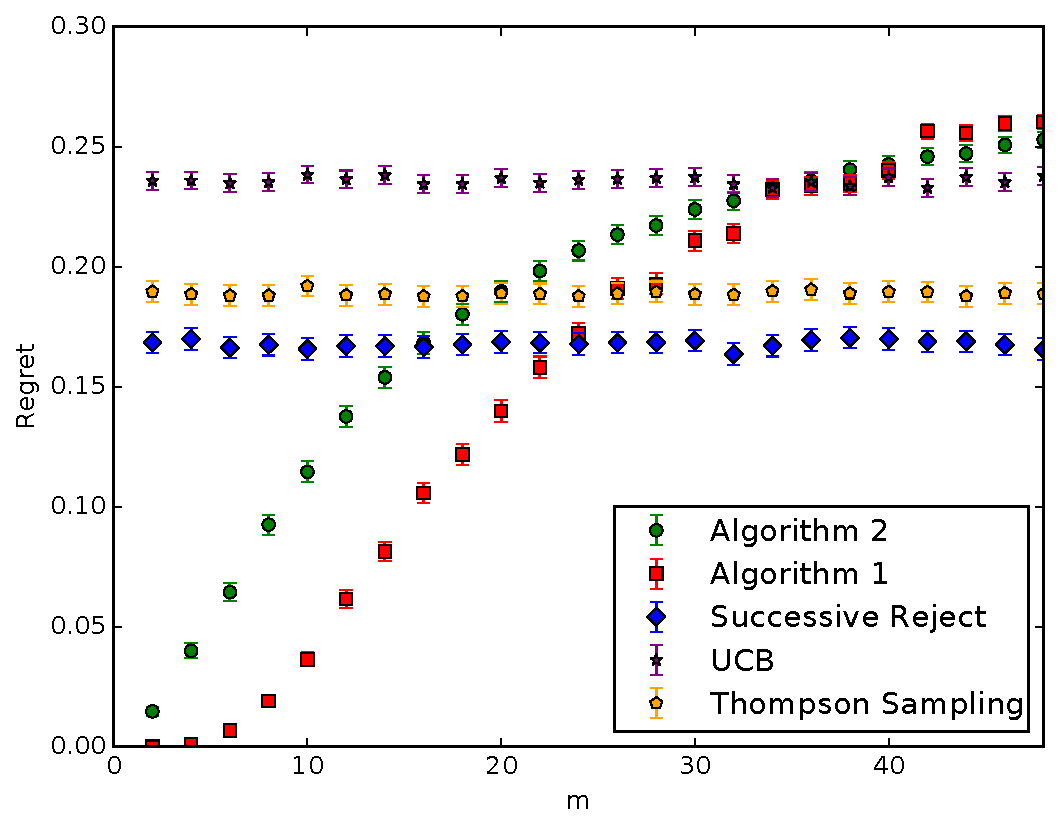
\includegraphics[width=\textwidth]{experiment1_20161020_1247.pdf}
    		\caption{Simple regret vs $m(\boldsymbol{q})$ for fixed horizon $T=400$ and number of variables $N = 50$}
        \label{fig:simple_vs_m}
    \end{subfigure}\hfill
    \begin{subfigure}[t]{0.3\textwidth}
    		\centering
        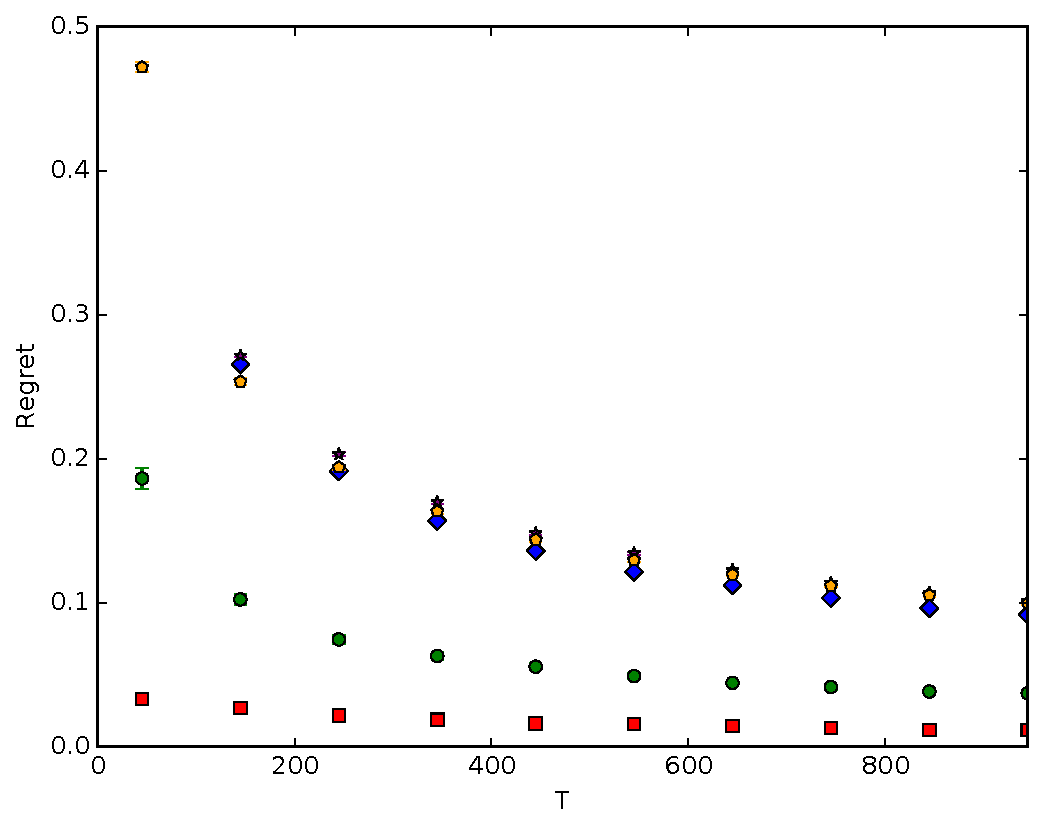
\includegraphics[width=\textwidth]{experiment2_20161020_1249.pdf}
    		\caption{Simple regret vs horizon, $T$, with $N = 50$, $m=2$ and $\epsilon = \sqrt{\frac{N}{8T}}$}
        \label{fig:simple_vs_T_vary_epsilon}
    \end{subfigure}\hfill
    \begin{subfigure}[t]{0.3\textwidth}
    		\centering
    		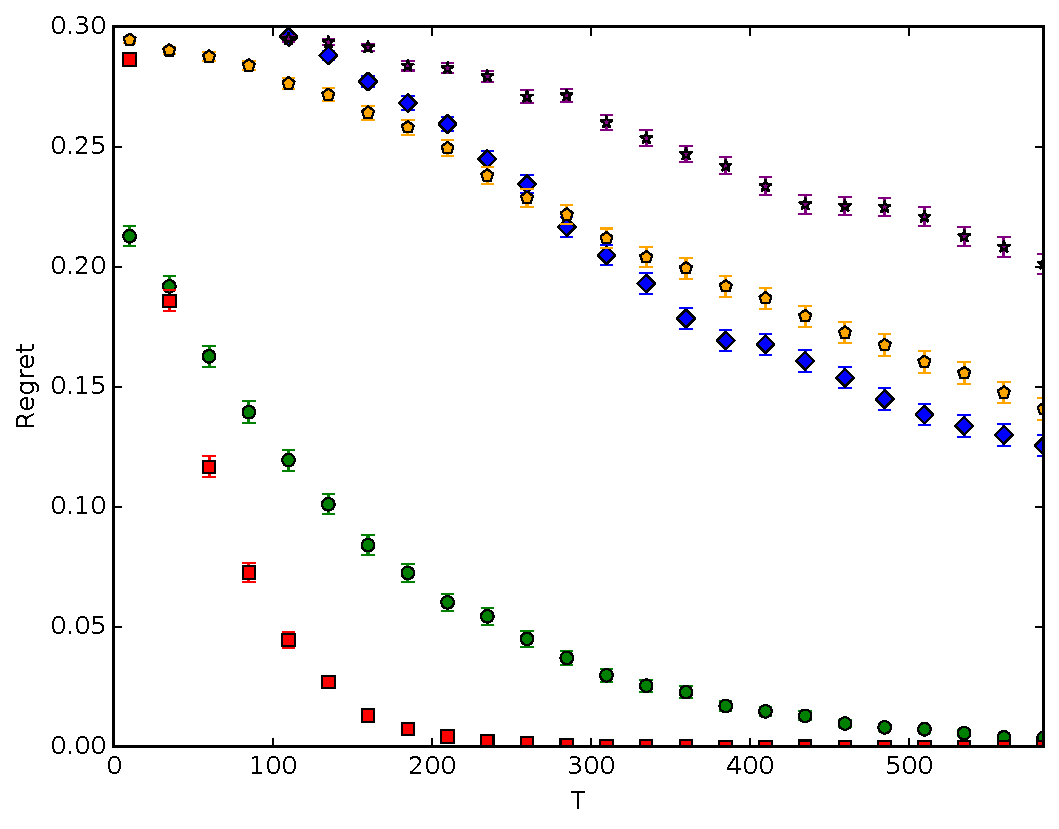
\includegraphics[width=\textwidth]{experiment3_20161020_1252.pdf}
    		\caption{Simple regret vs horizon, $T$, with $N = 50$, $m=2$ and fixed $\epsilon = .3$}
    		\label{fig:simple_vs_T}
    \end{subfigure}
    \caption{Experimental results}
    \label{fig:experiments}
\end{figure}

Figure \ref{fig:simple_vs_T_vary_epsilon} demonstrates the performance of the algorithms in the worst case environment for standard bandits, where the gap between the optimal and sub-optimal arms, $\smash{\epsilon = \sqrt{N/(8T)}}$ , is just too small to be learned. This gap is learnable by the causal algorithms, for which the worst case $\epsilon$ depends on $m \ll N$. In Figure \ref{fig:simple_vs_T} we fix $N$ and $\epsilon$ and observe that, for sufficiently large $T$, the regret decays exponentially. The decay constant is larger for the causal algorithms as they have observed a greater effective number of samples for a given $T$. 

For the parallel bandit problem, the regression estimator used in the specific algorithm outperforms the truncated importance weighted estimator in the more general algorithm, despite the fact the specific algorithm must estimate $\boldsymbol{q}$ from the data. 
This is an interesting phenomenon that has been noted before in off-policy evaluation where the regression (and not the importance weighted) estimator is known to be minimax optimal asymptotically \citep{LMS14}.


\subsection*{Additional experiments} \todo {tie section together}
\begin{figure}[H]
	\centering    
          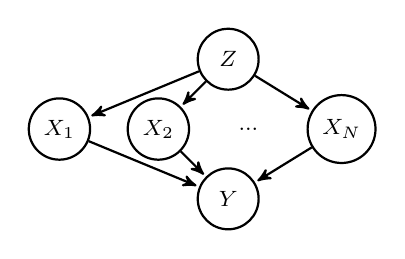
\begin{tikzpicture}[->,>=stealth',shorten >=1pt,auto,node distance=.45cm,
  thick,main node/.style={observed}, hidden/.style={empty},background rectangle/.style={fill=olive!45}]
%every node/.style={scale=0.6}
 %nodes
\node[main node](1){$X_{1}$};
\node[main node, right=of 1](2){$X_{2}$};
\node[hidden, right=of 2](3){$...$};
\node[main node, right=of 3](4){$X_{N}$};
\node[main node, below right=of 2](5){$Y$};
\node[main node, above right=of 2](6){$Z$};
 \path[every node/.style={font=\tiny}]
    (1) edge (5)
    	(2) edge (5)
    (4) edge (5)
    (6) edge (1) edge (2) edge (4);
\end{tikzpicture}
        \caption{Confounded graph}
        \label{fig:parallel_confounded} 
\end{figure}


We now compare the general algorithm with a range of standard bandit algorithms on the confounded graph in Figure \ref{fig:parallel_confounded}. All the variables are binary and the action space consists of the set of single variable interventions plus the do nothing action, $\calA = \set{\set{do(X_i = j)} \cup \set{do(Z = j)} \cup \set{do()}: 1\leq i \leq N,\; j \in \set{0,1}}$. We choose this setting because it generalises the parallel bandit, while simultaneously being sufficiently simple that we can compute the exact reward and interventional distributions for large $N$ (in general inference in graphical models is exponential in $N$). As before, we show the average regret over 10,000 simulations with error bars showing three standard errors. 

In Figure \ref{fig:simple_vs_m_general} we fix $N$ and $T$ and $P(Z=1) = .4$. For some $2 \leq N_1 \leq N$ we define 
\eq{
P(X_i = 1|Z = 0) &= \begin{cases} 0 & \text{ if } i \in \set{1,...N_1} \\ .4 & \text{ otherwise } \end{cases}\\
P(X_i = 1|Z = 1) &= \begin{cases} 0 & \text{ if } i \in \set{1,...N_1} \\ .65 & \text{ otherwise } \end{cases}
}
As in the parallel bandit case, we let $Y$ depend only on $X_1$, $P(Y|do(X_1=1)) = \frac{1}{2} + \epsilon$ and $P(Y|do(X_1=0)) = \frac{1}{2}-\epsilon'$, where $\epsilon' = \epsilon P(X_1=1) / P(X_1=0)$. The value of $N_1$ determines $m$ and ranges between $2$ and $N$. The values for the CPD's have been chosen such that the reward distribution is independent of $m$ and so that we can analytically calculate $\eta*$. This allows us to just show the dependence on $m$, removing the noise associated with different models selecting values for $\eta*$ with the same $m$ (and also worst case performance), but different performance for a given reward distribution. 

In Figure \ref{fig:simple_vs_T_general} we fix the model and number of variables, $N$, and vary the horizon $T$. $P(Z)$ and $P(X|Z)$ are the same as for the previous experiment.  
In Figure \ref{fig:simple_vs_T_misspecified} we additionally show the performance of Algorithm 1, but exclude actions on $Z$ from the set of allowable actions to demonstrate that Algorithm 1 can fail in the presence of a confounding variable, which occurs because it incorrectly assumes that $P(Y|do(X)) = P(Y|X)$. 
We let $P(Z) = .6$, $P(Y|\boldsymbol{X}) = X_7 \oplus X_N$ and $P(X|Z)$ be given by:

\eq{
P(X_i = 1|Z = 0) &= 
\begin{cases} 
.166 & \text{ if } i \in \set{1,..., 6} \\
.2 & \text{ if } i = 7 \\
.7 & \text { otherwise} 
 \end{cases}\\
 P(X_i = 1|Z = 1) &= 
\begin{cases} 
.166 & \text{ if } i \in \set{1,..., 6} \\
.8 & \text{ if } i = 7 \\
.3 & \text { otherwise} 
 \end{cases}\\
}

In this setting $X_7$ tends to agree with $Z$ and $X_N$ tends to disagree. It is sub-optimal to act on either $X_7$ or $X_N$, while all other actions are optimal. The first group of $X$ variables with $i \leq 6$ will be identified by the parallel bandit as the most unbalanced ones and played explicitly. All remaining variables are likely to be identified as balanced and estimated from observational estimates. The CPD values have been chosen to demonstrate the worst case outcome, where the bias in the estimates leads Algorithm 1 to asymptotically select a sub-optimal action.

\begin{figure}[H]
    \begin{subfigure}[t]{0.3\textwidth}
		\centering    
    		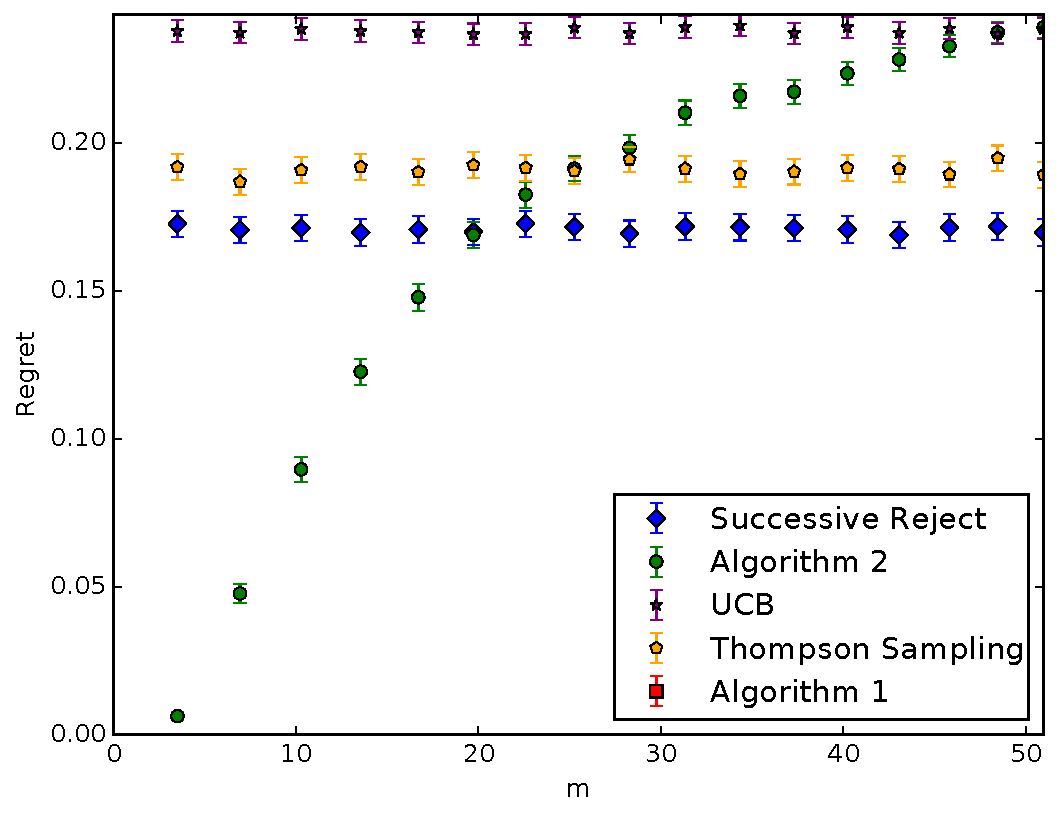
\includegraphics[width=\textwidth]{experiment4_20161023_2120.pdf}
    		\caption{Simple regret vs $m(\eta*)$ for fixed horizon $T=400$ and number of variables $N = 50$}
        \label{fig:simple_vs_m_general}
    \end{subfigure}\hfill
    \begin{subfigure}[t]{0.3\textwidth}
    		\centering
        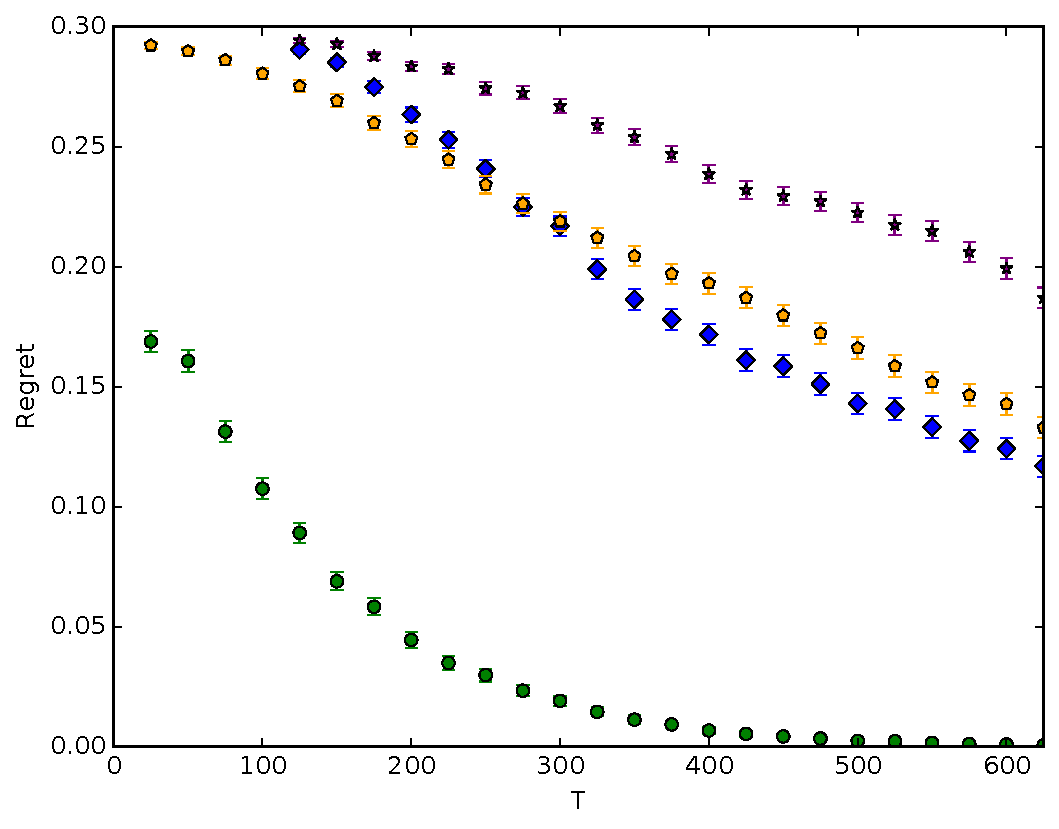
\includegraphics[width=\textwidth]{experiment7_20161020_1257.pdf}
    		\caption{Simple regret vs horizon, $T$, with $N = 50$ and $m(\eta*)=3.1$ }
        \label{fig:simple_vs_T_general}
    \end{subfigure}\hfill
    \begin{subfigure}[t]{0.3\textwidth}
    		\centering
    		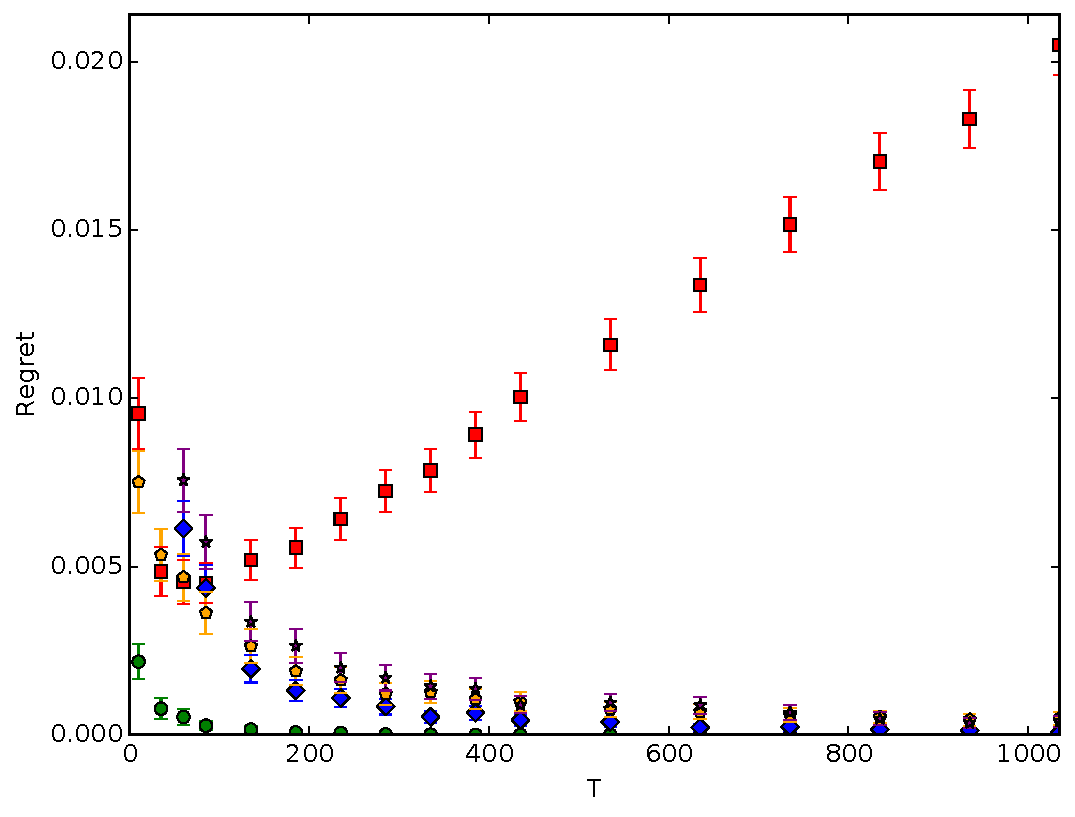
\includegraphics[width=\textwidth]{experiment5_20161023_2118.pdf}
    		\caption{Simple regret vs horizon, $T$, with $N = 21$, $m(\eta*)=4.3$ with no actions setting $Z$}
    		\label{fig:simple_vs_T_misspecified}
    \end{subfigure}
    \caption{Experimental results on the confounded graph}
    \label{fig:experiments_confounded}
\end{figure}

\subsection*{Discussion \& Future work}

Algorithm~\ref{alg:general} for general causal bandit problems 
estimates the reward for all allowable interventions $a \in \calA$ over $T$ rounds by sampling and applying interventions from a distribution $\eta$.
Theorem~\ref{thm:general} shows that this algorithm has (up to log factors) simple regret that is $\smash{\mathcal O(\sqrt{m(\eta)/T)}}$ where 
the parameter $m(\eta)$ measures the difficulty of learning the causal model and is always less than $N$.
The value of $m(\eta)$ is a uniform bound on the variance of the reward estimators $\hat{\mu}_a$ and, intuitively, problems where all variables' values in the causal model ``occur naturally'' when interventions are sampled from $\eta$ will have low values of $m(\eta)$.

The main practical drawback of Algorithm~\ref{alg:general} is that both the estimator $\hat{\mu}_a$ and the optimal sampling distribution $\eta^*$ (\ie, the one that minimises $m(\eta)$) require knowledge of the conditional distributions $\Pn{a}{\parents{Y}}$ for all $a \in \calA$. In contrast, in the special case of parallel bandits, Algorithm~\ref{alg:simple} uses the $do()$ action to effectively estimate $m(\eta)$ and the rewards then re-samples the interventions with variances that are not bound by $\hat{m}(\eta)$.
Despite these extra estimates, Theorem~\ref{thm:lower} shows that this approach is optimal (up to log factors).Finding an algorithm that only requires the causal graph and lower bounds for its simple regret in the general case is left as future work.


\paragraph{Making Better Use of the Reward Signal}
Existing algorithms for best arm identification are based on ``successive rejection'' (SR) of arms based on UCB-like bounds on their rewards~\citep{Even-Dar2002}. In contrast, our algorithms completely ignore the reward signal when developing their arm sampling policies and only use the rewards when estimating $\hat{\mu}_a$. Incorporating the reward signal into our sampling techniques or designing more adaptive reward estimators that focus on high reward interventions is an obvious next step. This would likely improve the poor performance of our causal algorithm relative to the sucessive rejects algorithm for large $m$, as seen in Figure~\ref{fig:simple_vs_m}.

For the parallel bandit the required modifications should be quite straightforward. The idea would be to adapt the algorithm to essentially use successive elimination in the second phase so arms are eliminated as soon as they are provably no longer optimal with high probability. In the general case a similar modification is also possible by dividing the budget $T$ into phases and optimising the sampling distribution $\eta$, eliminating arms when their confidence intervals are no longer overlapping. Note that these modifications will not improve the minimax regret, which at least for the parallel bandit is already optimal. For this reason we prefer to emphasize the main point that causal structure should be exploited when available. Another observation is that Algorithm \ref{alg:general} is actually using a fixed design, which in some cases may be preferred to a sequential design for logistical reasons. This is not possible for Algorithm \ref{alg:simple}, since the $\vec{q}$ vector is unknown.


\paragraph{Cumulative Regret}
Although we have focused on simple regret in our analysis, it would also be natural to consider the cumulative regret. In the case of the parallel bandit problem we can slightly modify the analysis from \citep{wu2015online} on bandits with side information 
to get near-optimal cumulative regret guarantees. They consider a finite-armed bandit model with side information where in reach round the learner chooses an action and receives a Gaussian reward signal for all actions, but with a known variance that depends on the chosen action. In this way the learner can gain information about actions it does not take with varying levels of accuracy. The reduction follows by substituting the importance weighted estimators in place of the Gaussian reward. In the case that $\vec{q}$ is known this would lead to a known variance and the only (insignificant) difference is the Bernoulli noise model. In the parallel bandit case we believe this would lead to near-optimal cumulative regret,
at least asymptotically. 

%Their model assumes the rewards for all arms $a$ are Gaussian with mean $\mu_a$ and variance $\sigma^2_{ab}$ and that playing an arm $a$ will reveal a side observation $Y_{ab}$ of the reward for all arms $b$ distributed with mean $\mu_b$ and variance $\sigma^2_{ab}$.
%We can build a similar dependence structure with variances for a Bernoulli reward variable that is derived from the $\vec{q}$ vector of probabilities.
%\todom{Check this!}
%Even though the original results are for Gaussian rewards we believe the analysis will go through largely unchanged.

The parallel bandit problem can also be viewed as an instance of a time varying graph feedback problem \citep{Alon2015,Kocak2014}, where at each timestep the feedback graph $G_t$ is selected stochastically, dependent on $\boldsymbol{q}$, and revealed after an action has been chosen. The feedback graph is distinct from the causal graph. A link $A \rightarrow B$ in $G_t$ indicates that selecting the action $A$ reveals the reward for action $B$. For this parallel bandit problem, $G_t$ will always be a star graph with the action $do()$ connected to half the remaining actions. However, \citet{Alon2015,Kocak2014} give adversarial algorithms, which when applied to the parallel bandit problem obtain the standard bandit regret. A malicious adversary can select the same graph each time, such that the rewards for half the arms are never revealed by the informative action. This is equivalent to a nominally stochastic selection of feedback graph where $\boldsymbol{q} = \boldsymbol{0}$. 

\cite{Lelarge2012} consider a stochastic version of the graph feedback problem, but with a fixed graph available to the algorithm before it must select an action. In addition, their algorithm is not optimal for all graph structures and fails, in particular, to provide improvements for star like graphs as in our case. \cite{Buccapatnam2014} improve the dependence of the algorithm on the graph structure but still assume the graph is fixed and available to the algorithm before the action is selected. 



\paragraph{Causal Models with Non-Observable Variables}
If we assume knowledge of the conditional \textit{interventional} distributions $\Pn{a}{\parents{Y}}$ our analysis applies unchanged to the case of causal models with 
non-observable variables. Some of the interventional distributions may be non-identifiable meaning we can not obtain prior estimates for $\Pn{a}{\parents{Y}}$ from 
even an infinite amount of observational data. Even if all variables are observable and the graph is known, if the conditional distributions are unknown, then Algorithm
\ref{alg:general} cannot be used. Estimating these quantities while simultaneously minimising the simple regret is an interesting and challenging open problem.

% For example, if we had access to a data set of \textit{experiments} in which the reward variable $Y$ was not available from which to build estimates of $P_a$.
% In this case, some conditional distributions may be non-identifiable. 
% The corresponding actions can be immediately added to the set $A$ prior to collecting any data. 
% We can then use the same algorithm as in the case where there are no latent variables, except that we will have to use the more general do-calculus rather than simply adjusting for the parents to write the expression for each action in terms of observational data.
% Combining our estimation techniques with insights from \citet{Bareinboim2015} for handling unobserved confounders would be worth investigation.


% More generally, assuming causal structure creates more complex types of side information, such as that shown in equation \ref{eq:estimation_transfer}. In this case, selecting one action does not fully reveal an alternate action but provides some information towards an estimate. The quality of the estimate notably depends not only on the number of times that action was selected. For example, to get a good estimate for $X_1 = 1$ by intervening on $X_2$ requires us to sample both $X_2=0$ and $X_2=1$, in proportions dependent on $q_2$. This more complex side information does not fit within the graph feedback framework.


\paragraph{Partially or Completely Unknown Causal Graph}
A much more difficult generalisation would be to consider causal bandit problems where the causal graph is completely unknown or known to be a member of class of models.
The latter case arises naturally if we assume free access to a large observational dataset, from which the Markov equivalence class can be found via causal discovery techniques. 
Work on the problem of selecting experiments to discover the correct causal graph from within a Markov equivalence class~\cite{Eberhardt2005,eberhardt2010causal,hauser2014two,Hu2014b} could potentially be incorporated into a causal bandit algorithm.
In particular, \citet{Hu2014b} show that only $\bigo{\log \log n}$ multi-variable interventions are required on average to recover a causal graph over $n$ variables once purely observational data is used to recover the ``essential graph''.
Simultaneously learning a completely unknown causal model while estimating the rewards of interventions without a large observational dataset would be much more challenging.




\chapter*{Causality in Marketing}
\section*{Attribution}
\section*{Econometric Modelling}

\chapter*{Conclusions (1000 words)}

\section*{Open questions}
\paragraph{Cycles} - a huge issue. Not covered by Pearl,Rubin etc. 

Places to look, statistical control theory, etc. any interesting papers along these lines?


\bibliographystyle{apalike}% Select the citation style e.g. ieeetr
\bibliography{../library}% write the directory to the .bib file
\end{document}




